% sage_latex_guidelines.tex V1.20, 14 January 2017
\documentclass[Royal,sagev,times]{sagej}

%make boxes
%https://texblog.org/2015/09/30/fancy-boxes-for-theorem-lemma-and-proof-with-mdframed/
\usepackage[framemethod=TikZ]{mdframed}
\usepackage{float}

\newcounter{Example}\setcounter{Example}{0}
\renewcommand{\thetheo}{\arabic{Example}}
\newenvironment{Example}[2][]{%
\refstepcounter{Example}%
\ifstrempty{#1}%
{\mdfsetup{%
frametitle={%
\tikz[baseline=(current bounding box.east),outer sep=0pt]
\node[anchor=east,rectangle,fill=black!20]
{\strut Box~\thetheo};}}
}%
{\mdfsetup{%
frametitle={%
\tikz[baseline=(current bounding box.east),outer sep=0pt]
\node[anchor=east,rectangle,fill=black!20]
{\strut Box~\thetheo:~#1};}}%
}%
\mdfsetup{innertopmargin=10pt,linecolor=black!20,%
linewidth=2pt,topline=true,%
frametitleaboveskip=\dimexpr-\ht\strutbox\relax
}
\begin{mdframed}[]\relax%
\label{#2}}{\end{mdframed}}

%
\usepackage{moreverb,url}

\usepackage[colorlinks,bookmarksopen,bookmarksnumbered,citecolor=red,urlcolor=red]{hyperref}

\newcommand\BibTeX{{\rmfamily B\kern-.05em \textsc{i\kern-.025em b}\kern-.08em
T\kern-.1667em\lower.7ex\hbox{E}\kern-.125emX}}

%\usepackage[
%backend=biber,style=numeric, autocite=superscript, sorting=none
%]{biblatex}

%\addbibresource{BIBTEXfile.bib} %Imports bibliography file

\def\volumeyear{2016}

\setcounter{secnumdepth}{3} 
\begin{document}

\begin{large}

{\fontfamily{ptm}\selectfont

\:
\:

\noindent Research Master’s programme \newline
Methodology \& Statistics for the Behavioural,  Biomedical \& Social Sciences \newline
Utrecht University, the Netherlands \\[4\baselineskip]

\noindent MSc Thesis Joukje Willemsen (4257634) \newline
Shortcomings of the test-then-pool method and equivalence testing as a more appropriate method of including historical controls \newline
May 2020 \\[4\baselineskip]

\noindent Supervisors: \newline
Dr. Katrien Oude Rengerink \newline
Prof. Dr. Kit C.B. Roes \\[2\baselineskip]

\noindent Second Grader: \newline
Dr. Daniel L. Oberski \\[4\baselineskip]

\noindent Preferred journal of publication: Statistical Methods in Medical Research \newline
Word count: 8042
}

\end{large}

\newpage 

% acknowledgement
% statement of interest
% 

%%% author surnames
\runninghead{Willemsen}

\title{Shortcomings of the test-then-pool method and equivalence testing as a more appropriate method of including historical controls}

%Incorporating historical controls in confirmatory clinical trials using frequentist methods that comprise equivalence testing}

%%% Authors %%%%
\author{Joukje Willemsen \affilnum{1}}%, Katrien Oude-Rengerink\affilnum{2} and Kit Roes\affilnum{3}}

\affiliation{
\affilnum{1} Utrecht University, Utrecht}\\
%\affilnum{2} Julius Centre, Utrecht\\
%\affilnam{3} Julius Centre, Utrecht}

\corrauth{Joukje Willemsen}
\email{j.e.willemsen@uu.nl}

\begin{abstract}
Including historical controls in the analysis of a new study can potentially improve power and lead to better parameter estimates. However, the assumption that the historical controls come from the same sampling distribution should be tested carefully to prevent bias and type I error inflation. Currently, this assumption is often tested with a test-than-pool (TTP) test that aims to detect a significant difference in estimated parameters. However, we reason that an equivalence test would be a better fit for this problem. Furthermore, we stress that only including historical controls that are very similar results in a form of confirmation bias. Bootstrapping is considered as a possible solution for this problem. Both the TTP method and the new proposed pooling methods are evaluated in a simulation study considering multiple scenarios that could be realistic in practice. The results show that equivalence testing indeed outperforms the regular TTP test. The equivalence methods where the confidence intervals are bootstrapped underperformed the other methods. Furthermore, the results show that even in a "perfect world scenario", the type I error rate is inflated for every pooling method. This is a problem that will remain an important issue when considering pooling historical controls in a current study.  
\end{abstract}

\keywords{Historical controls, Test-then-pool, equivalence testing, bootstrapping, pooling}

\maketitle
\section{Introduction}
The succes of randomised controlled trials (RCT) is reliant on a sufficient number of eligible participants.\cite{huang2018Recruitment} Unfortunately, according to a study of 114 UK trials in all health care contexts, less than a third (31\%) of the included trials achieved their original recruitment target.\cite{mcdonald2006} Despite efforts over multiple decades to make patient recruitment more successful, the recruitment problem remains.\cite{huang2018Recruitment} At the same time, RCT data is accumulating and more accessible than ever.\cite{dejardin2018} Ideally, previous relevant information would be incorporated into future trials to reduce the required sample size of future trials.
%Especially in read diseases

%\subsubsection{Historical controls}
Data of previous trials performed within a similar setting are often available.\cite{vRosmalen2018} Even though the evaluated treatment in the experimental groups usually differs between trials among the same target population, the treatment (or lack of treatment) in the control groups is often the same.\cite{vRosmalen2018} We call the controls in these previous studies "historical controls" when the control-population in the previous trial are eligible for inclusion in the analysis of a (hypothethical) new trial, or "current trial".\cite{vRosmalen2018} Historical controls should be chosen carefully, to ensure sufficient comparability with  the current trial.\cite{vRosmalen2018}

Ideally, the historical controls and the current controls are sampled from the same population. In this case, pooling would in the long run increase power and provide better estimates. Unfortunately, in practice we are faced with the uncertainty of drift in the control population.\cite{viele2014} A few potential differences between the current and historical controls are listed in table \ref{Table:differences}. 

\begin{table}[h!]
%\small\sf\centering
\caption{Potential differences between current controls and historical controls.\cite{simmons2009} \label{Table:differences}}
\begin{tabular}{l}
\toprule
$\bullet$ Regional differences in care, environmental factors and gene pools.\\
$\bullet$ Prognosis may differ as a result of differences in care and support. \\
$\bullet$ Selection bias as a result of the consent requirements. \\ 
$\bullet$ Data for the two groups may differ with respect to completeness or quality. \\
$\bullet$ Patients may have been diagnosed at a different point of their illness. \\
\bottomrule
\end{tabular}\\[10pt]
\end{table}
Differences in patient populations or other trial-specific circumstances can lead to heterogeneity among the historical trials and the current trial, \cite{vRosmalen2018} inducing bias and type I error inflation.\cite{viele2014} To test the assumption that the historical controls and current controls are sufficiently comparable, both Bayesian and frequentist methods have been proposed. 

\paragraph{Bayesian methods}
The idea that there is useful information contained within historical data available prior to a clinical trial fits perfectly with the Bayesian paradigm of updating current knowledge with new data.\cite{lim2018} However, despite tremendous effort, the reconciliation of the formulation of the hypotheses and the calculation of type I error between a Bayesian analysis and traditional frequentist analysis remains unclear.\cite{quan2019} Therefore, one may be cautious of Bayesian approaches for incorporating historical controls into confirmatory trials.\cite{lim2018} To ensure that including historical information will be accepted by regulatory authorities and adopted by clinical researchers, a statistical approach that has reasonable frequentist properties is needed.\cite{normington2019} Most importantly, it is necessary that the type I error rate is controlled - at least in all scenarios that are realistic in practice.\cite{Mielke2018}

%%%
%%
%%
% is needed afzwakken naar iets softers

\paragraph{Frequentist test-then-pool method}
Viele et al. described a simple approach to determine whether historical data should be included in a new trial based on the equality of the historical and new - or "current" - control group. \cite{vRosmalen2018} This two-step approach consists of performing a frequentist test to test the null hypothesis that the two control groups originate from the same distribution.\cite{viele2014} If the null hypothesis of equality is not rejected, it is assumed that the two groups are homogeneous can be pooled. If the hypothesis of equality is rejected, the historical controls are ignored. \cite{viele2014} The final analysis is performed without the inclusion of historical controls. This test-then-pool (TTP) method has been described, evaluated and applied in multiple articles. The test is straightforward; the researcher only has to specify a critical $p$-value; $\alpha$. However, this method has a few shortcomings.

First, a nonsignificant difference may not always imply consistency between the historical and current information.\cite{li2020} The TTP is designed to make decisions about a difference in outcome, indicated by a small $p$-value.\cite{Silva2009} When the $p$-value is large, it is concluded that there is no difference. However, "absence of evidence is not evidence of absence"*\cite{altman1995}. When a null hypothesis significance test fails to reject the null-hypothesis this can be either due to a lack of power to detect a difference or truly no difference.\cite{Silva2009} Even the smallest deviation can be detected if the power is high enough, resulting in a significant $p$-value. Not having enough power to detect a difference should not be a valid reason to pool. At the same time, a statistical difference does not indicate clinical relevance.\cite{kruschke2018} When the difference between the two groups is too small to be of any clinical relevance, it should not stop the researcher from pooling the control groups.

Secondly, although for the test-then-pool method the researcher does not explicitly specify how much difference between the two groups should or should not be tolerated, such a threshold is indirectly determined by a combination of the power of the test and the specified $\alpha$. This means that the threshold of tolerated difference is hard to predict, calculate, communicate and replicate.\cite{kruschke2018} An illustration of this problem is presented in box \ref{thm:threeresearchers}.

\begin{Example}[Reproducability of the difference threshold\label{thm:threeresearchers}]

Consider the following three researchers and the characteristics of their current control groups.\\

\begin{tabular}{|{2cm}|P{2cm}|P{2cm}|}
\hline
Researcher & SE & sample size\\
\hline
A & 20 & 100\\
B & 10 & 100\\
C & 10 & 200\\
\hline
\end{tabular}
\\
The true underlying difference between the current and historical control group is equal for every researcher. If all three researchers would apply a TTP to their data with the same $\alpha$, the indirectly specified difference threshold would be different for all of them. Researcher A would most likely be allowed to pool according to the test, because the TTP difference test is least likely to find an effect. Researcher C would be least likely be allowed to pool according to the test, because the TTP difference test is most likely to find an effect. In essence, researcher A is punished for having more power.
\end{Example}\\

Preferably we would have a test where the decision threshold for "maximum allowed difference" would be set directly, and not be mindlessly dictated by a combination of power and $\alpha$. This would require the researcher to actively think about what difference would be clinically relevant. Specifying these thresholds directly would promote transparency and replicability. As proposed by Li, Liu and Snavely in their recent article,\cite{li2020} an equivalence test might be a better fit for this kind of problem. Where traditional (two-sided) significance testing designs focus on demonstrating a difference between groups, equivalence testing designs test whether or not two groups are practically equivalent.\cite{walker2011}\\

\paragraph{Equivalence testing}
In the frequentist hypothesis testing framework, it is statistically impossible to support the hypothesis that a true effect size is exactly zero.\cite{lakens2017} However, it is possible to assert that the true difference ($\delta_{c-h}$) is unlikely to be outside a certain range by testing for equivalence.\cite{jones1996} Equivalence between two treatments can be tested by comparing the constructed $100(1-2\alpha)\%$ confidence interval (CI) for the parameter of interest ($\delta_{c-h}$) with a pre-specified "range of practical equivalence",\cite{koti2013} as is further explained in box \ref{box:eq}. In the case of pooling historical and current controls, the question of interest is not whether we can conclude that there is a difference between the two groups, but whether we can conclude that the two groups are not clinically and statistically different from each other.\cite{greene2008} \\

\begin{Example}[Equivalence testing \label{box:eq}]

The "range of equivalence" indicates a range of effect sizes or values that would not be considered a clinically relevant difference+\cite{walker2011} the parameter of interest is close enough to the null value to be considered equivalent.\cite{walker2011} The range of equivalence is compared with the confidence interval to make an inference about the equivalence of the two control groups.\cite{lakens2017} When the confidence interval is contained within the range of equivalence, we can conclude that the groups are practically equivalent.\cite{dienes2016} A difference between the two control groups is concluded when the CI is entirely outside the range of equivalence. If the interval falls neither fully inside or outside the equivalence region, more power is required and no decision can be made. In the context of pooling, we should only pool when the CI is contained within the range of equivalence.
\end{Example}

However, one unlucky paradox remains: current controls that would benefit the most from pooling - because the parameter estimate is far away from the population parameter - have the least chance of getting pooled. If a current control group is a very unlucky sample,  pooling will probably help to obtain better estimates of the population distribution and therefore reduce bias. However, both a difference test and an equivalence test will most likely conclude that the groups are too different to get pooled. This results in only pooling that are very alike, a phenomenon that we will refer to as "cherry picking". To illustrate this problem, consider the following thought experiment: a researcher has performed a clinical study (referred to as current study) and has an infinite pool of historical control groups to choose from. If the researcher only pools those control groups that have the same estimated parameter, pooling the control groups will not lead to a better approximation of the population parameter. If the researcher very restrictively selected samples that are like your sample, (s)he could as well have copy-pasted the current controls to increase his sample size immediately. Cherry picking leads to confirmation bias: the standard errors are underestimated what results in increased false positive rates.

%%%%%%%%%%%%%%%%%%%%%%%%%%%%%%
% CONFIRMATION BIAS TOEVOEGEN
%%%%%%%%%%%%%%%%%%%%%%%%%%%%%%
\paragraph{Bootstrapping}
To avoid cherry picking we would ideally compare the underlying sampling distributions of the control groups to determine whether pooling is appropriate or not. When the samples are drawn from the same distribution, pooling will most likely pull the sample mean closer to the population mean. Although the sampling distribution is not known, we can estimate it using bootstrapping techniques.\cite{kulesa2015}\cite{koti2013} By applying a nonparametric bootstrap, the sampling distribution is approximated by randomly sampling with replacement from the observed data to obtain new samples of the same size.\cite{kulesa2015} Hence, equivalence tests that use bootstrapping to obtain the CI will be evaluated as a possible solution to the cherry-picking problem.

\paragraph{Study aim}
In this article equivalence testing is evaluated as a more appropriate measure for testing whether control groups are similar enough to pool. Whereas Li, Liu and Snavely\cite{li2020} mainly focus on normally distributed and dichotomous data, in this article the focus will be on survival data that follows a Weibull distribution. While Li, Liu and Snavely\cite{li2020} derive the type I error and power for the equivalence and difference test analytically, we performed a simulation study to compare the operating characteristics of both the TTP and different equivalent tests. Furthermore, bootstrapped CIs is considered as a possible solution to the cherry-picking problem. To test these hypotheses, a simulation study considering real-world historical controls is performed with simulated survival data to evaluate the operating characteristics of the new proposed methods and the difference (TTP) method. In the remainder of the article a working example and conceptual framework will be introduced before we elaborate on the details of the simulation study.

\section{Working example}
As a working example we will consider a hypothetical current trial that aims to test the effectiveness of a new treatment for amyotraphic lateral sclerosis (ALS). ALS is a rare devastating neurodegenerative disease for which there is currently no cure.\cite{han2017} Riluzole is the only FDA-approved treatment for ALS.\cite{han2017} Riluzole has been shown to prolong the median survival time by only 2 to 3 months in ALS patients.\cite{han2017} Researchers face the problem that there is a relatively small pool of ALS patients, limited financial resources, and a relatively large number of potential treatments for testing.\cite{simmons2009} Incorporating historical controls to make the ALS trials more resource-efficient may provide a solution to this problem.\cite{donofrio2011} Including historical controls in ALS clinical trials has already been done in practice. For example: Statland et al. enriched their randomized, double-blind, placebo-controlled trial of ALS participants with historical controls to test the effectiveness of Rasagiline.\cite{statland2019} The PRO-ACT data set (see box \ref{thm:pro-act}) provides data from patients that participated in previous trials. 
According to Atassi et al., the PRO-ACT database could serve as a source of well-matched historical controls for ALS trials.\cite{atassi2014} Using different pooling methods, it will be evaluated whether these historical controls can be pooled with (simulated) current controls in the hypothetical trial. With the resulting control group - pooled or not pooled - the effectiveness of the hypothetical new treatment based on the observed difference between the control group and experimental group is tested.


\begin{Example}[The PRO-ACT dataset \label{thm:pro-act}]
A
ALS is a rare disease with an annual incidence of 2/100,000.\cite{atassi2014} Because of this, clinical trials have typically been relatively small and aggregation of studies is needed to allow enough statistical power to answer important questions about the natural history and clinical symptoms of ALS.\cite{atassi2014} The Pooled Resource Open-Access ALS Clinical Trials (PRO-ACT) database has been designed and made publicly available to provide a solution to this problem.\cite{atassi2014} The dataset is the largest aggregation of ALS clinical trial data available. Currently, sixteen phase II and III ALS trials and one large observational study, conducted over the past 2 decades are included. The goal of the PRO-ACT database is to facilitate research that might leverage its remarkable statistical power for meaningful disease insights. Further details about how the data is obtained can be found in the article of Atassi et al..\cite{atassi2014}
\end{Example}

\section{Conceptual framework}
In this section theoretical background is discussed regarding modeling and testing survival data that applies to our working example. The expected effect of pooling in different scenarios is discussed. In tabel \ref{Abbreviations} the frequently used abbreviations and symbols used in this article are presented for reference.

\begin{table}[H]
%\small\sf\centering
\caption{Frequently used symbols and abbreviations\label{Abbreviations}}
\begin{tabular}{lll}
\toprule
Abbreviation&&\\
\midrule
$\lambda$&scale parameter of the Weibull distribution\\ 
$\gamma$&shape parameter of the Weibull distribution\\ 
_c & (current) control group \\
_e & experimental group \\
_{h} & historical controls \\
$\sigma^2_{\epsilon_{s}}$ & between-study variance parameter\\
RMST&Restricted Mean Survival Time\\ 
FPR&False Positive Rate\\ 
TPR&True Positive Rate\\ 
ROC curve& Receiver Operating Characteristics curve\\
\bottomrule
\end{tabular}\\[10pt]
\end{table}

\subsection{ Modeling survival time}
Clinical trials commonly record the length of time from study entry to a disease endpoint (death in case of survival data) for a treatment and a control group.\cite{spruance2004} The time between study entry and the participants death is called survival time.\cite{crumer2011} According to van Eijk et al. time-to-event data in ALS clinical trials are best modeled using Weibull distributions.\cite{van2019} The Weibull model is a popular parametric model for survival times as it is a very flexible model.\cite{crumer2011} The probability to survive upto a certain time point under a Weibull distribution is given by:
\begin{equation}\label{eq:Survival}
S(t)=\exp(-\lambda t^\gamma)
\end{equation}
.\cite{crumer2011}\cite{van2019}
Where t is time, $\lambda$ is the scale parameter and $\gamma$ is the shape parameter. When $\gamma = 1$, the Weibull distribution becomes the exponential distribution and the hazard rate remains constant.\cite{crumer2011} When $\gamma > 1$, the hazard rate increases with time, meaning that the instantaneous risk of dying increases with time.\cite{crumer2011} When $\gamma < 1$, the hazard rate decreases with time, meaning that the instantaneous risk of dying becomes less with time .\cite{crumer2011} The scale parameter $\lambda$ has an effect on the scale or "stretch" of the distribution. Consider $t_A$ and $t_B$ where $S(t_A) = 0$ and $S(t_B) = 1$. The difference $t_B - t_A$ is dictated by $\lambda$.

\subsection{Testing survival data}
For the analysis of our working example we consider two different statistical tests for survival data: the more conventional hazard ratio (HR) test and the nonparametric Restricted Mean Survival Time (RMST) test.

\subsubsection{HR test}
There are several methods available to analyze time-to-event curves.\cite{spruance2004} The Cox proportional hazards model has been the most popular popular procedure for many years in medical research.\cite{spruance2004}

The hazard ratio is simply calculated as:
\begin{equation}
    {HR_{ce}}(t) = \frac{h(t|\lambda_c)}{h(t|\lambda_e)}
\end{equation}.\cite{spruance2004} 

where $h(t|\lambda_c)$ and $h(t|\lambda_e)$ are the hazard rates of the control groups and experimental groups at time $t$ respectively. When calculating the hazard ratio it is assumed that the shape parameter $\gamma$ in equation \ref{eq:Survival} is the same in the control group and experimental group. It is assumed that the treatment effect of the experimental groups and the non-commensurability between control groups depend on the scale parameter $\lambda$ only:
\begin{equation}\label{eq:hazardrates}
\frac{h(t|\lambda_c = \beta_0)}{h(t|\lambda_e = \beta_0 + \beta_1)}= \frac{\gamma exp{(\beta_0)}t^{\gamma-1}}
{\gamma exp{(\beta_0+\beta_1)}t^{\gamma-1}} = exp{(-\beta_1)}
\end{equation} .\cite{crumer2011}

Where $h(t|\lambda_c = \beta_0)$ is the hazard rate of the control group, and $h(t|\lambda_e = \beta_0 + \beta_1)$ is the hazard rate of the experimental group. The resulting hazard rate $exp{(\beta_1)}$ is not a function of $t$ .\cite{crumer2011} 
\\

As becomes clear in equation \ref{eq:Survival} and equation \ref{eq:hazardrates}, when the proportional hazard assumption does not hold ($\gamma_c$ \neq $\gamma_e$), the scale parameter alone no longer captures the difference in survival time. Hence when the hazard ratio is not constant over time, meaning that the underlying proportional hazard assumption is violated, the ratio estimate is difficult or even impossible to interpret. \cite{huang2018RMST}

\subsubsection{Restricted Mean Survival Time}
An alternative parametric to capture the difference in survival time is a RMST test.\cite{huang2018RMST}
RMST is a robust and clinically interpretable summary measure of the survival time and is estimable even under heavy censoring $t_{cens}$.\cite{huang2018RMST} The RMST can be derived as the area under the curve $S_{(t)}$ from $t=0$ to $t=t_{cens}$

\begin{equation}
{\mu(t_{cens}) = \int_0^{t_{cens}} \! S(t) dt
}
\end{equation}.\cite{huang2018RMST}
To obtain an estimation of $\mu(t_{cens})$, $S(t)$ can be approximated with the Kaplan-Meier estimator for the survival function of T .\cite{huang2018RMST} The difference in RMST for an experimental group and control group can be estimated as
\begin{equation}
{ \hat{\mu}_e(t_{cens}) - \hat{\mu}_c(t_{cens})= \int_0^{t_{cens}} \! [\hat{S}_e(t)-\hat{S}_c(t)] dt
}
\end{equation}.\cite{huang2018RMST}

Alternatively, analogous to the HR, the ratio of RMST between groups can be used to indicate a difference in survival;
\begin{equation}
\frac{\int_0^{t_{cens}} \! \hat{S}_e(t) dt}{\int_0^{t_{cens}} \! \hat{S}_c(t) dt}
\end{equation}.\cite{huang2018RMST}

However, because the difference in RMST between two groups is easier to interpret and is clinically meaningful to characterize the treatment effect over time,\cite{huang2018RMST} this article will proceed only focusing on the direct difference in RMST, not the relative difference.\\

\subsection{The effect of pooling}
As stated by the central limit theorem, when we would repeatedly draw a random sample from the target population, register the survival times and use the data to estimate the Weibull scale-parameters of the control and experimental group
($\hat{\lambda_c}$ and $\hat{\lambda_e}$ respectively), the estimated scale parameters should approximate a normal distribution.\cite{koti2013} 
\begin{equation}
\hat{\lambda_c} \sim \mathcal{N}(\lambda_{c}, \frac{\sigma_{c}}{\sqrt{n_c}}) \end{equation}
\begin{equation}
\hat{\lambda_e} \sim \mathcal{N}(\lambda_{e}, \frac{\sigma_{e}}{\sqrt{n_e}}) 
\end{equation}
The mean of this distribution should equal the scale parameter that generated the data $\lambda_c$ and $\lambda_e$ respectively, while the variance of the distribution is a function of the variance on person level (between-person variance) and the number of samples $n$. 

In order to arrive at an accurate verdict about the effect of the treatment in the experimental group, ideally we would know how long the patients in the experimental group would have survived without the experimental treatment. Under the null-hypothesis (there's no effect) $\lambda_{c}=\lambda_{e}$ and $\sigma_{c}=\sigma_{e}$. Hence, when there is no effect present in the experimental group, and the sample size $n$ is equal, the sampling distribution of the experimental group and sampling distribution of the control group should overlap. The control group in a randomized controlled trial provides an estimate of what would have been the disease progression or survival times of the participants in the experimental group under $H_0$. Including historical controls in the study can either improve this estimation or induce bias. In the next two paragraphs, six different scenarios (that are referred to as scenario A - F) and the long-run effects of including historical controls in the study are discussed.

\subsubsection{When $\gamma_{h}$ = $\gamma_{c}$ is assumed}
The best guess for the scale parameter we would have observed from the experimental group under the null hypothesis ($\hat{\lambda}_e|H_0$) is $\lambda_c$, which we try to estimate with $\hat{\lambda}_c$. Pooling only affects the estimated scale parameter of the control group, $\hat{\lambda_c}$. Pooling can pull $\hat{\lambda_c}$ closer to $\hat{\lambda}_e|H_0$ or draw it further away from it. 

In figure \ref{fig:A-D}, the sampling distributions of the historical control, current control and experimental group are visualized for four scenarios, A-D, which are introduced in the following paragraphs.\\

\begin{figure}[H]
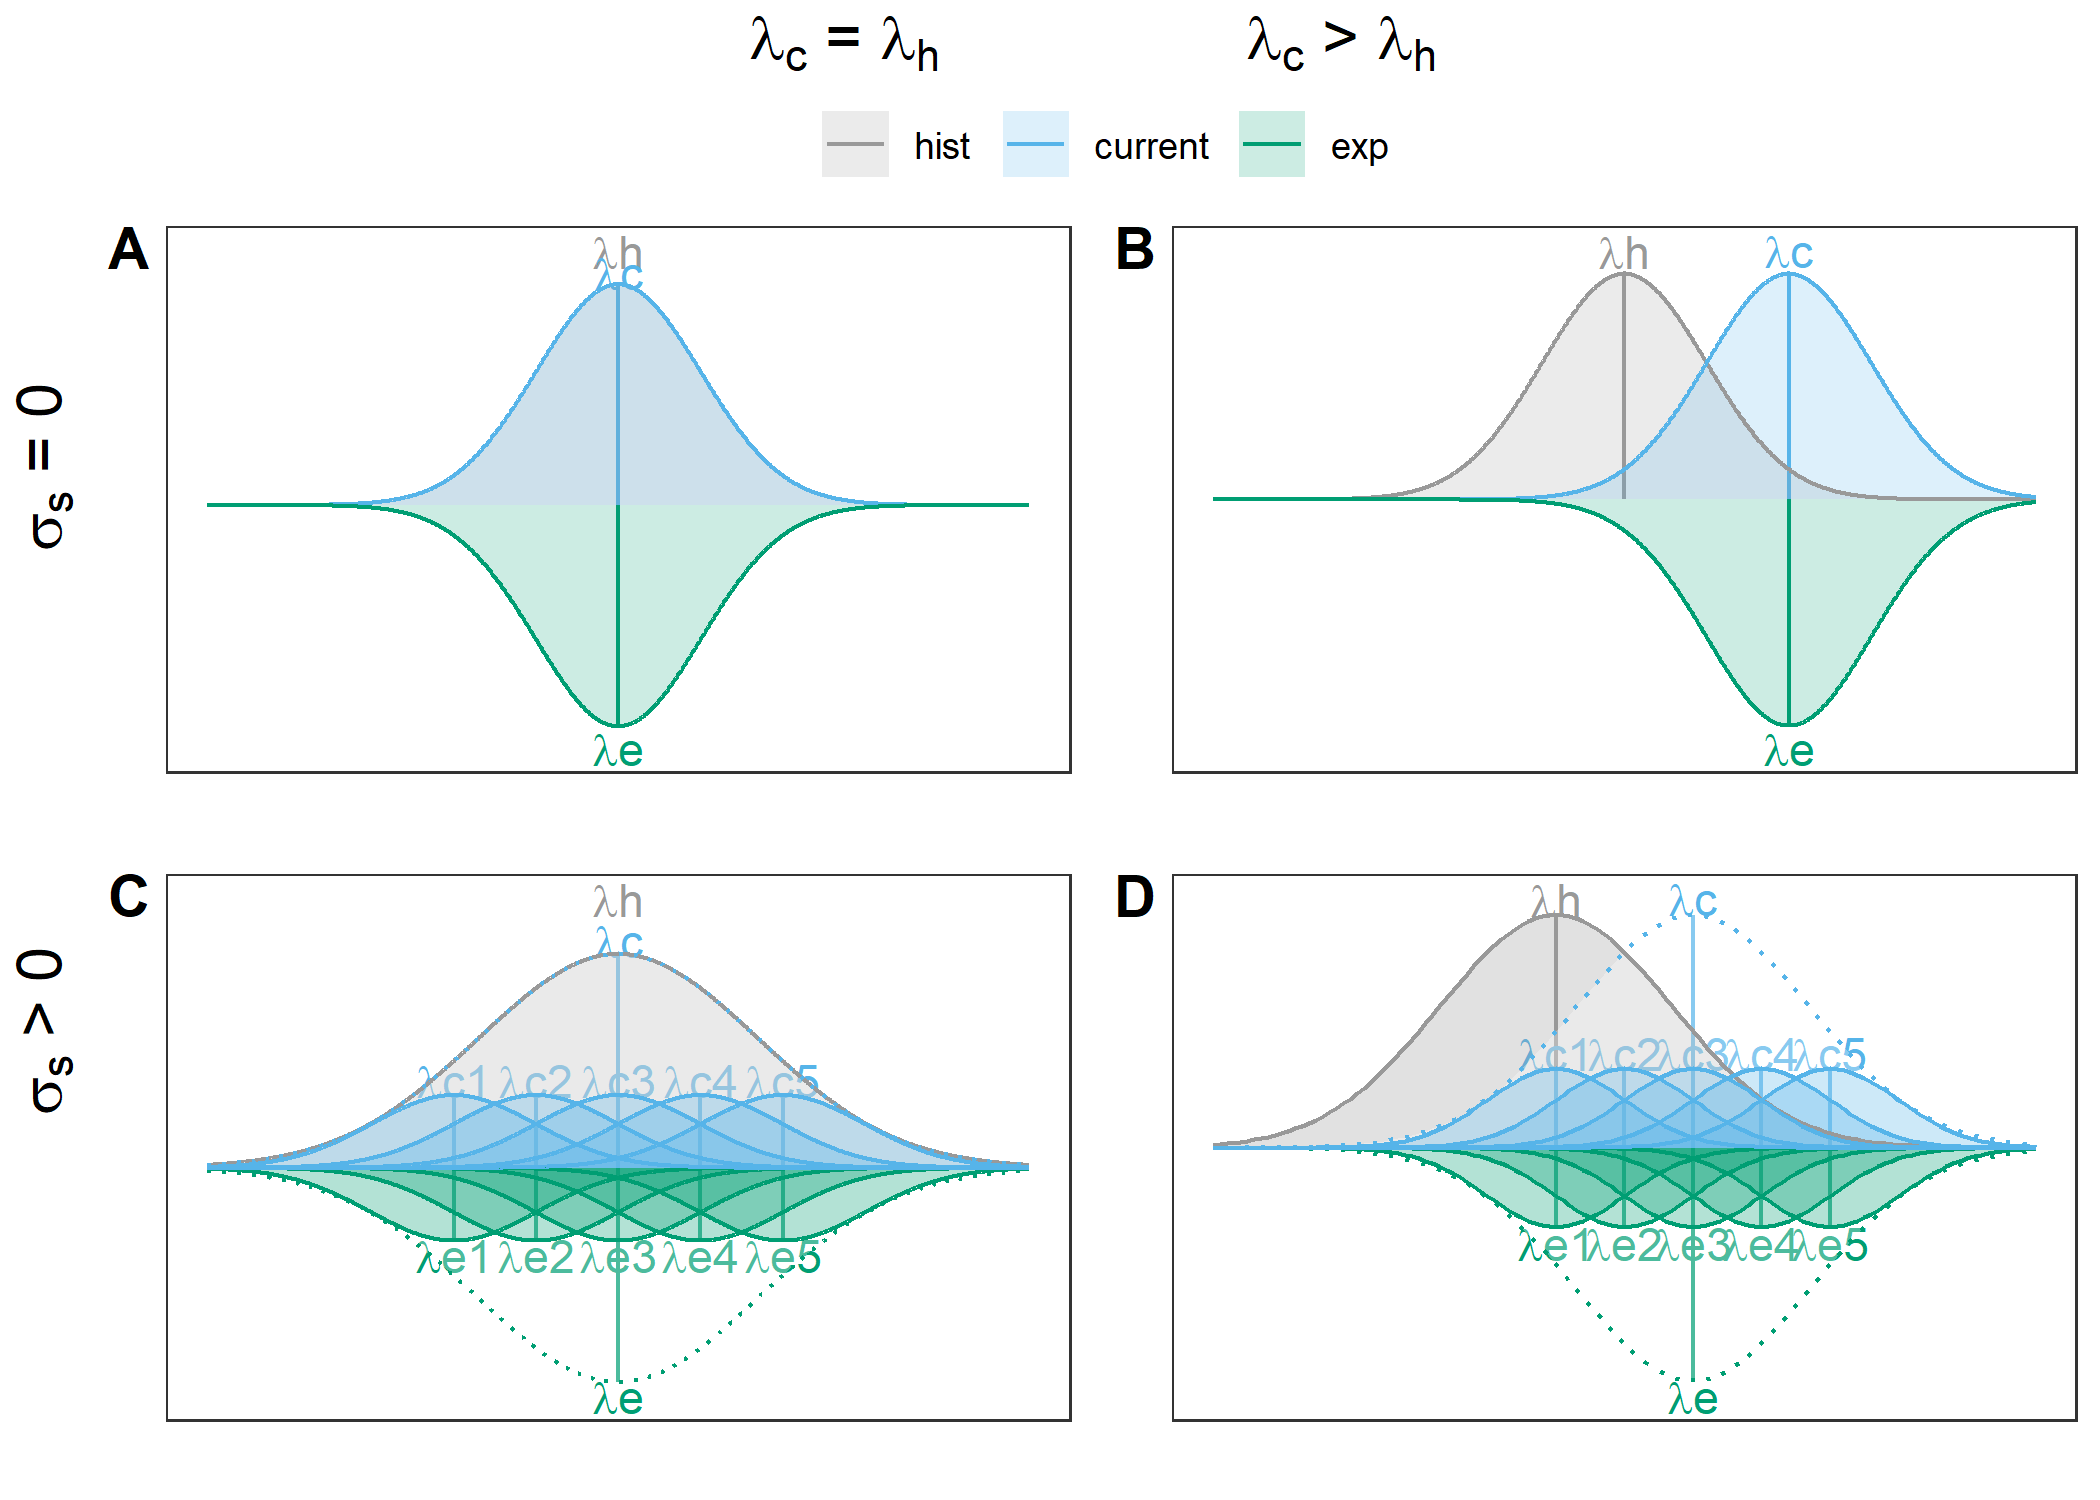
\includegraphics[width=12cm]{ScenarioABCD.png}
  \caption{Scenario A, B, C and D: To illustrate the four scenarios, the sampling distributions of the historical control group, current control group and experimental control under the null hypothesis group are plotted. In the left column (A \& C), the scale population parameter of the current and historical control group are the same $\lambda_c = \lambda_{h}$. In the right column (B \& D) the scale population parameter of the current and historical control group are different $\lambda_c \neq \lambda_{h}$. In the first row (A \& B), there is no between-study variance. In the second row (C \& D) between-study variance is present.}
  \label{fig:1}
\end{figure}

A) Scenario A (figure \ref{fig:1}A) is a "perfect world scenario", where the control groups are fully commensurate ($\lambda_{c} = \lambda_{h}$), as visualized in figure \ref{fig:1}A. 

When the current control group and the historical control group are randomly sampled from the same population, the estimated parameters $\hat{\lambda_{c}}$ and $\hat{\lambda_{h}}$ should also come from the same sampling distribution:

\begin{equation}
\hat{\lambda_{c}}, \hat{\lambda_{h}}  \sim \mathcal{N}(\lambda_{c}, \frac{\sigma_{c}}{\sqrt{n_{c}}}) \end{equation}

In this situation, pooling would decrease the sampling error and most likely improve the estimate of $\lambda_c$ and therefore improve the estimate of $\hat{\lambda}_e|H_0$. This results in an increase in true positive rate (TPR, or power) and decrease the false positive rate (FPR, or type I error).\\

B) In scenario B (figure \ref{fig:1}B), the control groups are not commensurate ($\lambda_{c} \neq \lambda_{h}$). This would be the case when the two samples come from different sampling frames. For example when there are cohort differences between the current and historical patients. For the scenario visualized in figure \ref{fig:1}B, pooling would draw $\hat{\lambda_c}$ towards $\lambda_{h}$, which is on average further away from $\lambda_{c}$ and $\hat{\lambda}_e|H_0$. This increases the FPR. The TPR will increase when pooling pulls $\hat{\lambda_c}$ further away from $\hat{\lambda}_e|H_1$, but decrease when pooling pulls $\hat{\lambda_c}$ closer to $\hat{\lambda}_e|H_1$.

This would increase both the FPR and TPR.\\

C) In scenario C (figure \ref{fig:1}C), multiple sample distributions with different means are plotted to indicate between study variance. The means of the sample distributions form their own overarching sample distribution, with means $\lambda_{e}$ and $\lambda_{c}$ as indicated in the plot. Because the PRO-ACT data set is the result of $23$ pooled studies and between study variance is present, the sampling distribution of the historical control group is assumed to be an accurate representation of the overarching sampling distribution. The means of the overarching sample distributions for the current control and experimental groups overlap with the sample mean of the historical control, indicating that the estimated scale parameters $\hat{\lambda}_{c}$ and $\hat{\lambda_e}|H_0$ are on average equal to $\lambda_{h}$. \\
It should be noted that, in order to make a fair comparison between the experimental group and the control group, in this case estimating $\lambda_{c}$ is not the goal. Instead, it is of interest to estimate $\lambda_{c_{i}}$; the mean of the sample distribution of the control group that also corresponds to the mean of the sample distribution of the experimental group $\lambda_{e_{i}}$ under $H_0$. In this case, pooling would only improve $\hat{\lambda_{c_{i}}}$ when $\lambda_{c_{i}}$=$\lambda_{h}$ (which is the case for $\lambda_{c3}$ in figure \ref{fig:1}C). In the other cases, pooling will on average increase the difference between $\hat{\lambda}_{ci}$ and $\lambda__{ci}$ and will therefore result in an increased FPR. The effect of pooling on the TPR depends on the direction of the effect. \\

D) In the fourth scenario (figure \ref{fig:1}D), the mean of the overarching sampling distribution of the current control group is not equal to the mean of the sampling distribution of the historical control group  $\lambda_{c}\neq\lambda_{h}$ and a between-study variance is present. In most cases, except for the sampling distribution with mean $\lambda_{c_1}$, pooling will pull the estimated scale parameter $\hat{\lambda_{c_{i}}}$ away from $\lambda_{c_{i}}$ and will therefore result in an increased FPR. The effect of pooling on the TPR depends on the direction of the effect.\\

\subsubsection{When $\gamma_{c}$ and $\gamma_{h}$ differ}
As visualized in figure \ref{fig:ScenarioA-F}, when both $\gamma_c$ and $\lambda_c$ are varied, the difference in survival time between the current controls and historical control is no longer directly related to $\lambda$. Although the simulated scenarios A and B, and E and F have the same scale parameters, their survival curves are different. 

Instead of considering the sampling distributions of the scale parameters $\lambda_c$ and $\lambda_{h}$ to make a decision about the pool-ability of two control groups, we will consider the sampling distributions of $RMST_{c}$ and $RMST_{h}$. The best guess for the RMST we would have observed from the experimental group under $H_0$ ($RMST_e|H_0$) is $RMST_c$, which we try to estimate with $\hat{RMST_c}$. Pooling only affects the estimated RMST of the control group $\hat{RMST_c}$. Pooling can pull $\hat{RMST_c}$ closer to $RMST_c$ or draw it further away from it.\\

E) In scenario E (figure \ref{fig:ScenarioA-F}E), $\lambda_{c} = \lambda_{h}$ and $\gamma_{c} > \gamma_{h}$. As can be inferred from equation \ref{eq:Survival} and figure \ref{fig:ScenarioA-F}, $RMST_{c} > RMST_{h}$. Pooling will pull $\hat{RMST}_{c}$ further away from $\hat{RMST_e}|H_0$. This leads to an increased FPR. When pooling pulls $\hat{RMST}_{c}$ further away from $\hat{RMST_e}|H_1$, pooling will increase the TPR. When pooling pulls $\hat{RMST}_{c}$ closer to $\hat{RMST_e}|H_1$, pooling will decrease the TPR. 

F) In the sixth scenario (figure \ref{fig:ScenarioA-F}E), $\lambda_{c} > \lambda_{h}$ and $\gamma_{c} > \gamma_{h}$. Consequently, $RMST_{c} > RMST_{h}$, as can be inferred from equation \ref{eq:Survival} and figure \ref{fig:ScenarioA-F}. Pooling will pull $\hat{RMST}_{c}$ further away from $\hat{RMST_e}|H_0$ as compared to scenario E.

\begin{figure}[h!] 
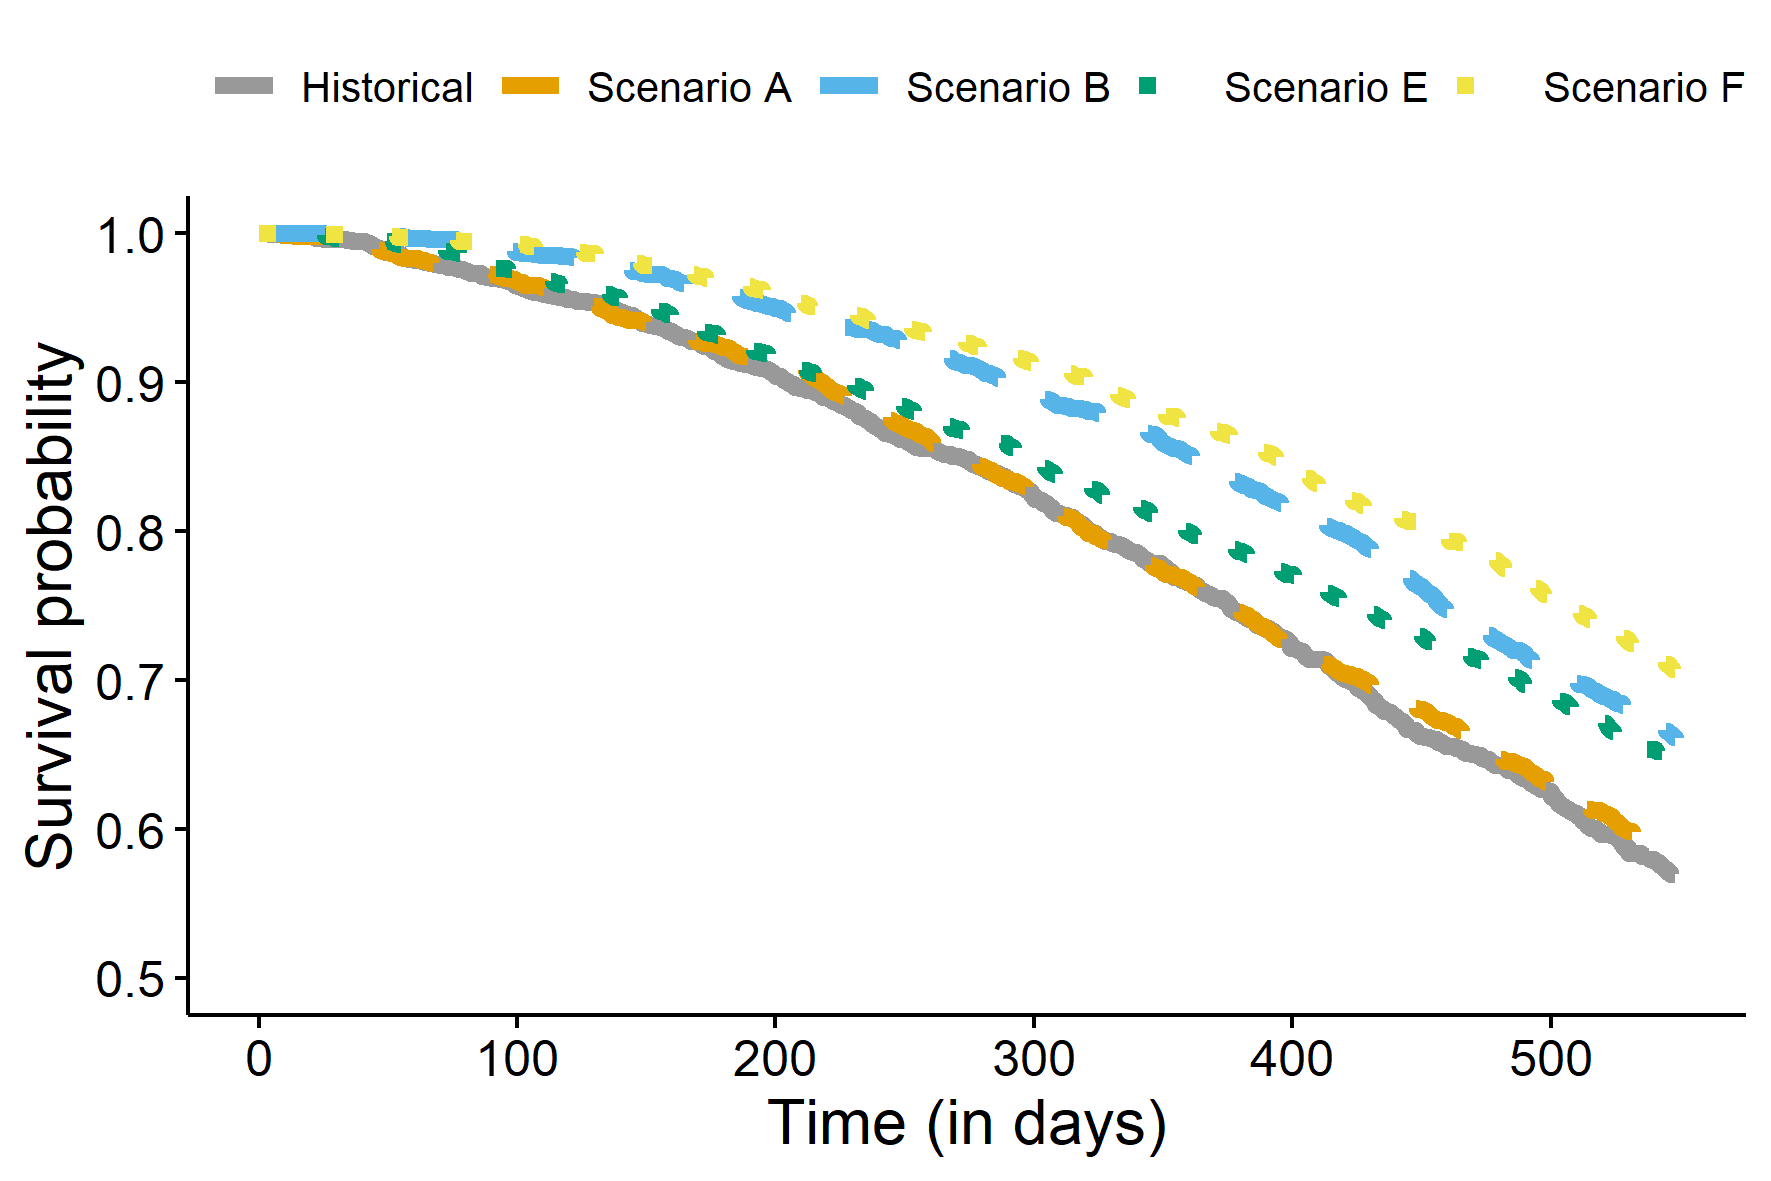
\includegraphics[width=12cm]{situaties.png}
  \caption{The survival curves of situation A, B, E and F. The survival probability is plotted on the y-axis, the x-axis indicates the time in days. The grey line indicates the survival curve of the historical controls. Scenario A is simulated such that $\gamma_c = \gamma_{h}$ and $\lambda_c = \lambda_{h}$ parameters as the historical control group. Scenario B is a simulated such that $\gamma_{c} = \gamma_{h}$ and $\lambda_{c} > \lambda_{h}$. Scenario E is simulated such that $\gamma_{c} > \gamma_{h}$ and $\lambda_{c} = \lambda_{h}$. Scenario F is simulated such that $\gamma_{c} > \gamma_{h}$ and $\lambda_{c} > \lambda_{h}$. Only scenario A results in a similar survival curve as the historical control group.}
  \label{fig:ScenarioA-F}
\end{figure}

\section{Simulation study}
To asses the decision quality of the pooling methods in different scenarios, the input parameters for $\lambda_{c}$, $\gamma_{c}$ and the between-study variance of $\lambda_{c}$ ($\sigma^2_{\epsilon_{s}}$) are varied across fourteen simulated control and experimental groups. The scenarios are categorised in 6 general scenarios, analogous to the scenarios A-F as presented in the previous section. The Rcode used to generate the data and perform the analysis is available on \href{https://github.com/JoukjeWillemsen/Research-Repository-Master-Thesis}{GitHub}. 

\subsection{Simulation settings}
The input parameters are simulated relative to a "perfect world scenario". In the perfect world scenario the historical controls and current controls come from the same distribution. To simulate this scenario, it was necessary to model the historical data in order to obtain input parameters for the current data. Therefore, the Weibull parameters from the historical (PRO-ACT) data were estimated using the function \textit{survreg} from the \textit{Survival} package \cite{survivalpackage}. The resulting values were transformed to fit the parameterization of the scale and shape according the to the built-in \textit{rweibull} function. This resulted in $\gamma_{h}$ = 1.68 and $\lambda_{h}$ = 776.89. Scenario A, the "perfect world scenario" is simulated such that $\gamma_{c} = \gamma_{h}$ and $\lambda_{c} = \lambda_{h}$ and the between study variance is $0$. The input parameters corresponding with the different situations as described in the previous section are listed in table \ref{T1}. 

\begin{table}[h!]
%\small\sf\centering
\caption{Simulated scenarios. The scenarios A, B, C and D correspond to the scenarios as visualized in Figure \ref{fig:1}. The scenarios A, B, E and F are visualized in figure \ref{fig:ScenarioA-F}\label{T1}}
\begin{tabular}{lllll}
\toprule
Scenario&$\gamma$&$\lambda_{c}$&$\sigma^2_{\epsilon_{s}}$\\
\midrule
A&1.68&776.89&0 \\ 
B&1.68&876.89&0 \\ 
C1-3&1.68&776.89&(1) 0.1; (2) 0.2; (3) 0.4\\ 
D1-3&1.68&876.89&(1) 0.1; (2) 0.2; (3) 0.4\\ 
E1-3&(1) 1.85; (2) 2.02; (3) 2.184 & 776.89 & 0\\ 
F1-3&(1) 1.85; (2) 2.02; (3) 2.184  & 876.89 & 0\\ 
\bottomrule
\end{tabular}\\[10pt]
\end{table}

\subsection{Sample size}
As discussed in the introduction, pooling historical controls could potentially help under-powered studies to reach a sufficient level of power. To illustrate this in our working example, the sample size of the simulated current study is set to equal a power of $60\%$ to detect an effect of HR = $0.5$ with $\alpha = 0.05$ without the inclusion of historical controls. An expected effect of HR = $0.5$ is realistic for an ALS clinical trial. According to van Eijk et al. who performed a systematic literature search and extracted design settings from 13 ALS clinical trials, the median expected treatment effect was $HR = 0.56$, ranging from [$0.33 - 0.66$].\cite{van2019}

The R-code in the source documentation for the TRICALS Time-to-Event module was used to perform the sample size calculation.\cite{van2019} This resulted in a required sample size of 68 in both the control group and experimental group; a total of 136.

\subsection{Simulation procedure}
For each scenario three data sets are simulated: a control group, an experimental group where HR = 0.5, to assess the TPR as well as an experimental group where HR = 1, to assess the false-positive-rate FPR. All the simulations are executed in Rstudio version 1.1.456,\cite{Rstudio} R version 3.6.2.\cite{Rmanual} The number of simulations for every simulated scenario as described in tabel \ref{T1} is 1000. 

If between-study variance is present, study effects are randomly generated by:

 \begin{equation}
 \epsilon_s \sim N (0,\sigma^2_{\epsilon_{s}}).
 \end{equation}. 
For every person $i$ in study $s$ survival time is randomly sampled from
%\begin{equation}
 %   T^{surv}_{is} \sim Weibull(\gamma,\lambda e^{-(\beta_s*X_{is}+\epsilon_s+\gamma})
%\end{equation}
\begin{equation}
    T^{surv}_{is} \sim Weibull(\gamma,\lambda_{c_s} e^{-(\beta_sX_{is})/\gamma})
\end{equation}
where
\begin{equation}
    \lambda_{c_s} = \lambda_c e^{-(\epsilon_s/\gamma)}
\end{equation}

The treatment effect of study $s$ is denoted by $\beta_s$, the dummy variable $X_{is}$ indicates whether person $i$ in study $s$ received treatment. Because most ALS-trials have a follow-up of 18 months (548 days) or less \cite{van2019} the survival time is censored at $T^{survival}_{is}>548$, indicated by a censoring indicator.

\subsection{Pooling methods}
\subsubsection{HR difference test}
A Cox proportional HR test is performed using the $coxph()$ function from the \textit{survival} package\cite{survivalpackage}. The $p$-value corresponding to the likelihood ratio test is extracted.
The historical and current control groups are only pooled when the $p$-value is bigger than the specified $\alpha$.

\subsubsection{HR equivalence test}
The CI of the the hazard ratio is calculated using the functions $coxph()$ and $Confint()$ from the \textit{Survival} package\cite{survivalpackage}. Equivalence is concluded when the 95\% CI is entirely between $HR_{lower bound}(t)$ and $HR_{upper bound}(t)=1/HR_{lower bound}(t)$.\cite{Silva2009}
The calculated CI is compared to the equivalence interval. The historical and current control groups are only pooled when the CI falls within the equivalence interval.  

\subsubsection{HR equivalence boot test}
Bootstrapping was performed using the $boot()$ function from the \textit{boot} package\cite{bootpackage} in R. The number of resamples is set at 400. For every bootstrapped sample, the hazard ratio is calculated $HR_{boot} = h_{c_{boot}}/h_{h}(t)$ using the function $coxph()$ from the \textit{Survival} package\cite{survivalpackage}. The bootstrap CI for the 95\% bootstrapped hazard ratios is obtained using the $boot.ci()$ function from the \textit{boot}\cite{bootpackage} package (using the "Normal" CI). 
The bootstrapped CI is compared to the equivalence interval. The historical and current control groups are only pooled when the bootstrapped CI falls within the equivalence interval. 

\subsubsection{RMST equivalence test}
$\hat{RMST}_hc$ and $SE(\hat{RMST})$ of the historical control group and simulated current control groups are obtained using the function $survmean()$ from the \textit{Survival} package.\cite{survivalpackage} The restricted time was set at 548, because most ALS-trials have a follow-up of 18 months (548 days) or less.\cite{van2019} The difference in RMST and the standard error of the estimate is simply calculated as
\begin{align*} \label{RMST CI}
\hat{\Delta} &= \hat{RMST_{c}} - \hat{RMST_{h}} \\
SE(\hat{\Delta}) &= \sqrt{SE(\hat{RMST_{c}})^2 + SE(\hat{RMST_{h}})^2}  \\
\end{align*}

.\cite{royston2013} The CI is calculated as

\begin{align*}
CI_{95\%} &= [\hat{\Delta}-1.96*SE(\hat{\Delta}) , \hat{\Delta}+1.96*SE(\hat{\Delta})]
\end{align*} .\cite{royston2013}
The calculated CI is compared to the equivalence interval. The historical and current control groups are only pooled when the bootstrapped CI falls within the equivalence interval.

\subsubsection{RMST equivalence boot test}
Bootstrapping was performed using the $boot()$ function from the \textit{boot} package in R.\cite{bootpackage} The number of resamples is set at 400. For every bootstrapped sample, the difference in restricted mean survival time is obtained using the function $survmean()$ from the \textit{Survival} package, with a restricted time of 548. For every bootstrapped sample $\hat{\Delta} = \hat{RMST_{c_{boot}}} - \hat{RMST_{h}}$ is calculated. The bootstrapped $95\%$ CI for \hat{$\Delta$} is obtained using the $boot.ci()$ function from the \textit{boot} package (using the "Normal" CI). 
The bootstrapped CI is compared to the equivalence interval. The historical and current control groups are only pooled when the bootstrapped CI falls within the equivalence interval.

\subsection{Decision thresholds}
The decision thresholds for every pooling method were set such that the extreme thresholds resulted in either "always pool" or "never pool", with many thresholds in between to cover the entire spectrum. A table with the applied thresholds can be found in Appendix \ref{A:Poolingcriteria}.

\subsection{Final analysis}
In order to obtain the FPR and TPR for every pooling method, a final analysis is conducted that tests for a difference in the (pooled or not pooled) control group and experimental group. The FPR is obtained by performing a difference test that compares the (pooled or not pooled) control group with an experimental group where no true effect is present (HR = 1). The TPR is obtained by performing a difference test with an experimental group where there is a true effect (HR = 0.5). Because the difference in decision qualities of the pooling methods could depend on the choice of the final analysis, the final analysis is performed twice; once with a Cox proportional Hazard ratio difference test and once with a RMST difference test.

\subsubsection{HR difference test}
A Cox proportional HR test is performed using the $coxph()$ function from the \textit{survival} package\cite{survivalpackage}. The $p$-value corresponding to the likelihood ratio test is extracted. The $p$-value is compared to $\alpha=0.05$. $p \leq \alpha$, indicates either a true positive or false positive, depending on the experimental group included in the analysis. 

\subsubsection{RMST difference test}
The $\hat{RMST}$ and $SE(\hat{RMST})$ of the (either pooled or not pooled) control group and the experimental groups are obtained using the function $survmean()$ from the \textit{Survival} package.\cite{survivalpackage} The restricted time was set at 548, because most ALS-trials have a follow-up of 18 months (548 days) or less.\cite{van2019} The difference in RMST and the standard error of the estimate is calculated as
\begin{align*} \label{RMST CI final}
\hat{\Delta} &= \hat{RMST_{e}} - \hat{RMST_{c}} \\
SE(\hat{\Delta}) &= \sqrt{SE(\hat{RMST_{e}})^2 + SE(\hat{RMST_{c}})^2} 
\end{align*}
.\cite{royston2013} $\hat{\Delta}/SE(\hat{\Delta})$ is compared to a standard normal distribution to test the null hypothesis $\Delta = 0$.\cite{royston2013} The $p$-value is compared with $\alpha=0.05$. $p \leq \alpha$, indicates either a true positive or false positive, depending on the experimental group included in the analysis. 

\subsection{Data analysis}
For every simulated control group (14 x 1000), the decision "pool" or "not pool" are saved for all the decision thresholds evaluated for all pooling methods. For every pooling methods and all the applied decision thresholds in each scenario the TPR (TP/(TP+FN)) and FPR (FP/(TP+FN)) is calculated over the 1000 datasets.\cite{hajian2013} 

\subsection{Data visualization}
To compare the operating characteristics of the pooling methods, the TPR and FPR is plotted for every pooling method and every decision threshold to resemble a receiver operating characteristic (ROC) curve. The ROC curve shows the trade-off between the true positive rate (sensitivity) and false positive rate (1 - sensitivity).\cite{hajian2013} One main advantage of using this method to compare the accuracy of the pooling methods is that the derived summary measure of accuracy does not depend on just one decision criterion.\cite{hajian2013} 
The thresholds all start at a point where you will never be able to pool ("never pool"), hence the TPR and FPR are the same as when you would ignore the historical data. Gradually, the thresholds become less strict to a point that we will refer to as "always pool". What happens in between those points is of interest; like a ROC-curve, the pooling method that lies closest to the top-left corner, has a better TPR/FPR trade-off. 

The TPR/FPR ratio is also plotted against the total proportion of pooled datasets to get a better insight in how the TPR/FPR ratio changes as the decision thresholds become less strict. These plots are presented in Appendix \ref{A:additionalgraphs}.

\section{Simulation results}
The results of the simulated scenarios C and D are presented in figure \ref{fig:A-D}, the simulated scenarios E and F are presented in figure \ref{fig:Sim2}. The results of the simulated scenarios A and B are presented in both figure \ref{fig:A-D} and \ref{fig:Sim2} as reference. The labels of the graphs correspond with the scenarios indicated in tabel \ref{T1}. In both graphs, the left two columns correspond with the operating characteristics obtained by performing a HR difference test as final analysis. The right two columns correspond with the operating characteristics obtained by performing a RMST difference test as final analysis. When interpreting the graphs, it should be noted that the scale of the x-axis and y-axis differ and vary among the graphs.

%Sim1
\begin{figure}[h!]
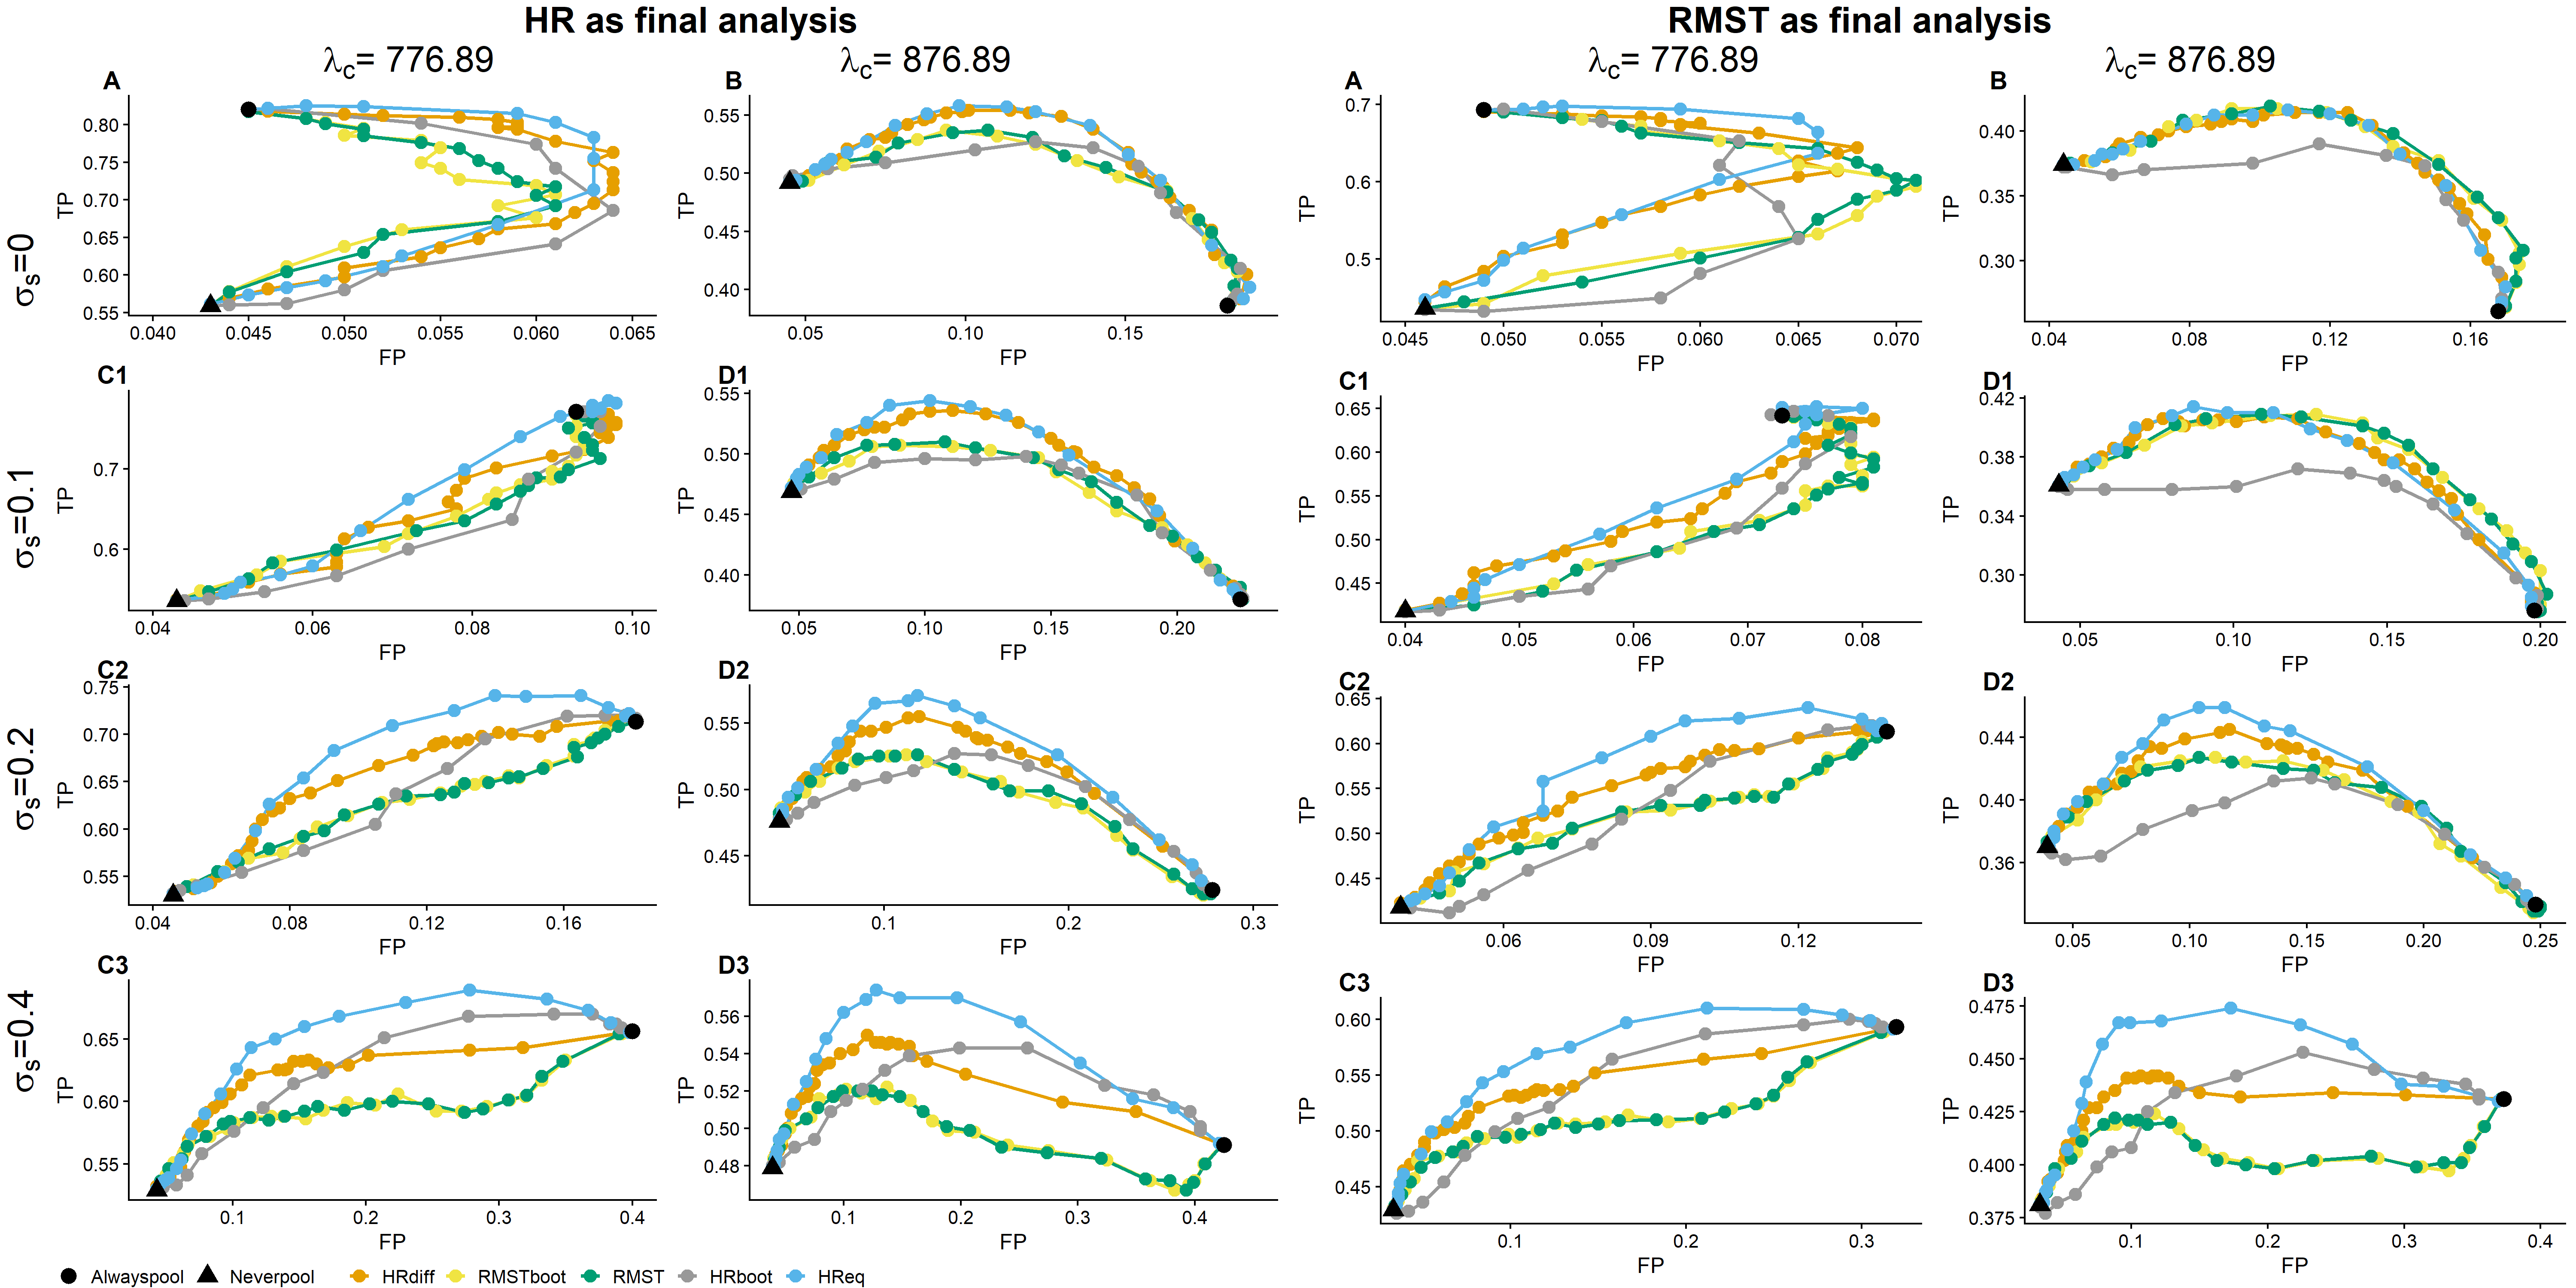
\includegraphics[width=13cm]{1.Sim1.png}
  \caption{Results scenario A-D: For the simulated scenarios A, B, C1-3 and D1-3, the TPR is plotted on the y-axis, the FPR is plotted for the six different pooling methods on the x-axis. It should be noted that the scale of the x-axis and y-axis differ and vary across the graph. The left two columns plot the operating characteristics when a HR is performed as final analysis, the right two columns plot the operating characteristics when a RMST is performed as final analysis. The input parameters for the different scenarios are indicated on the left and top of the figure. The graphs correspond to the scenarios described in table \ref{T1}, indicated in the left corner of every graph. The TPR/FPR trade-off in the situation "never pool" and "always pool" are indicated with $\triangle$ and $\bullet$ respectively.}
  \label{fig:A-D}
\end{figure}
%%%% AANPASSEN: BIJSCHRIFT & GROOTTE LEGENDA

%Sim1
\begin{figure}[h!]
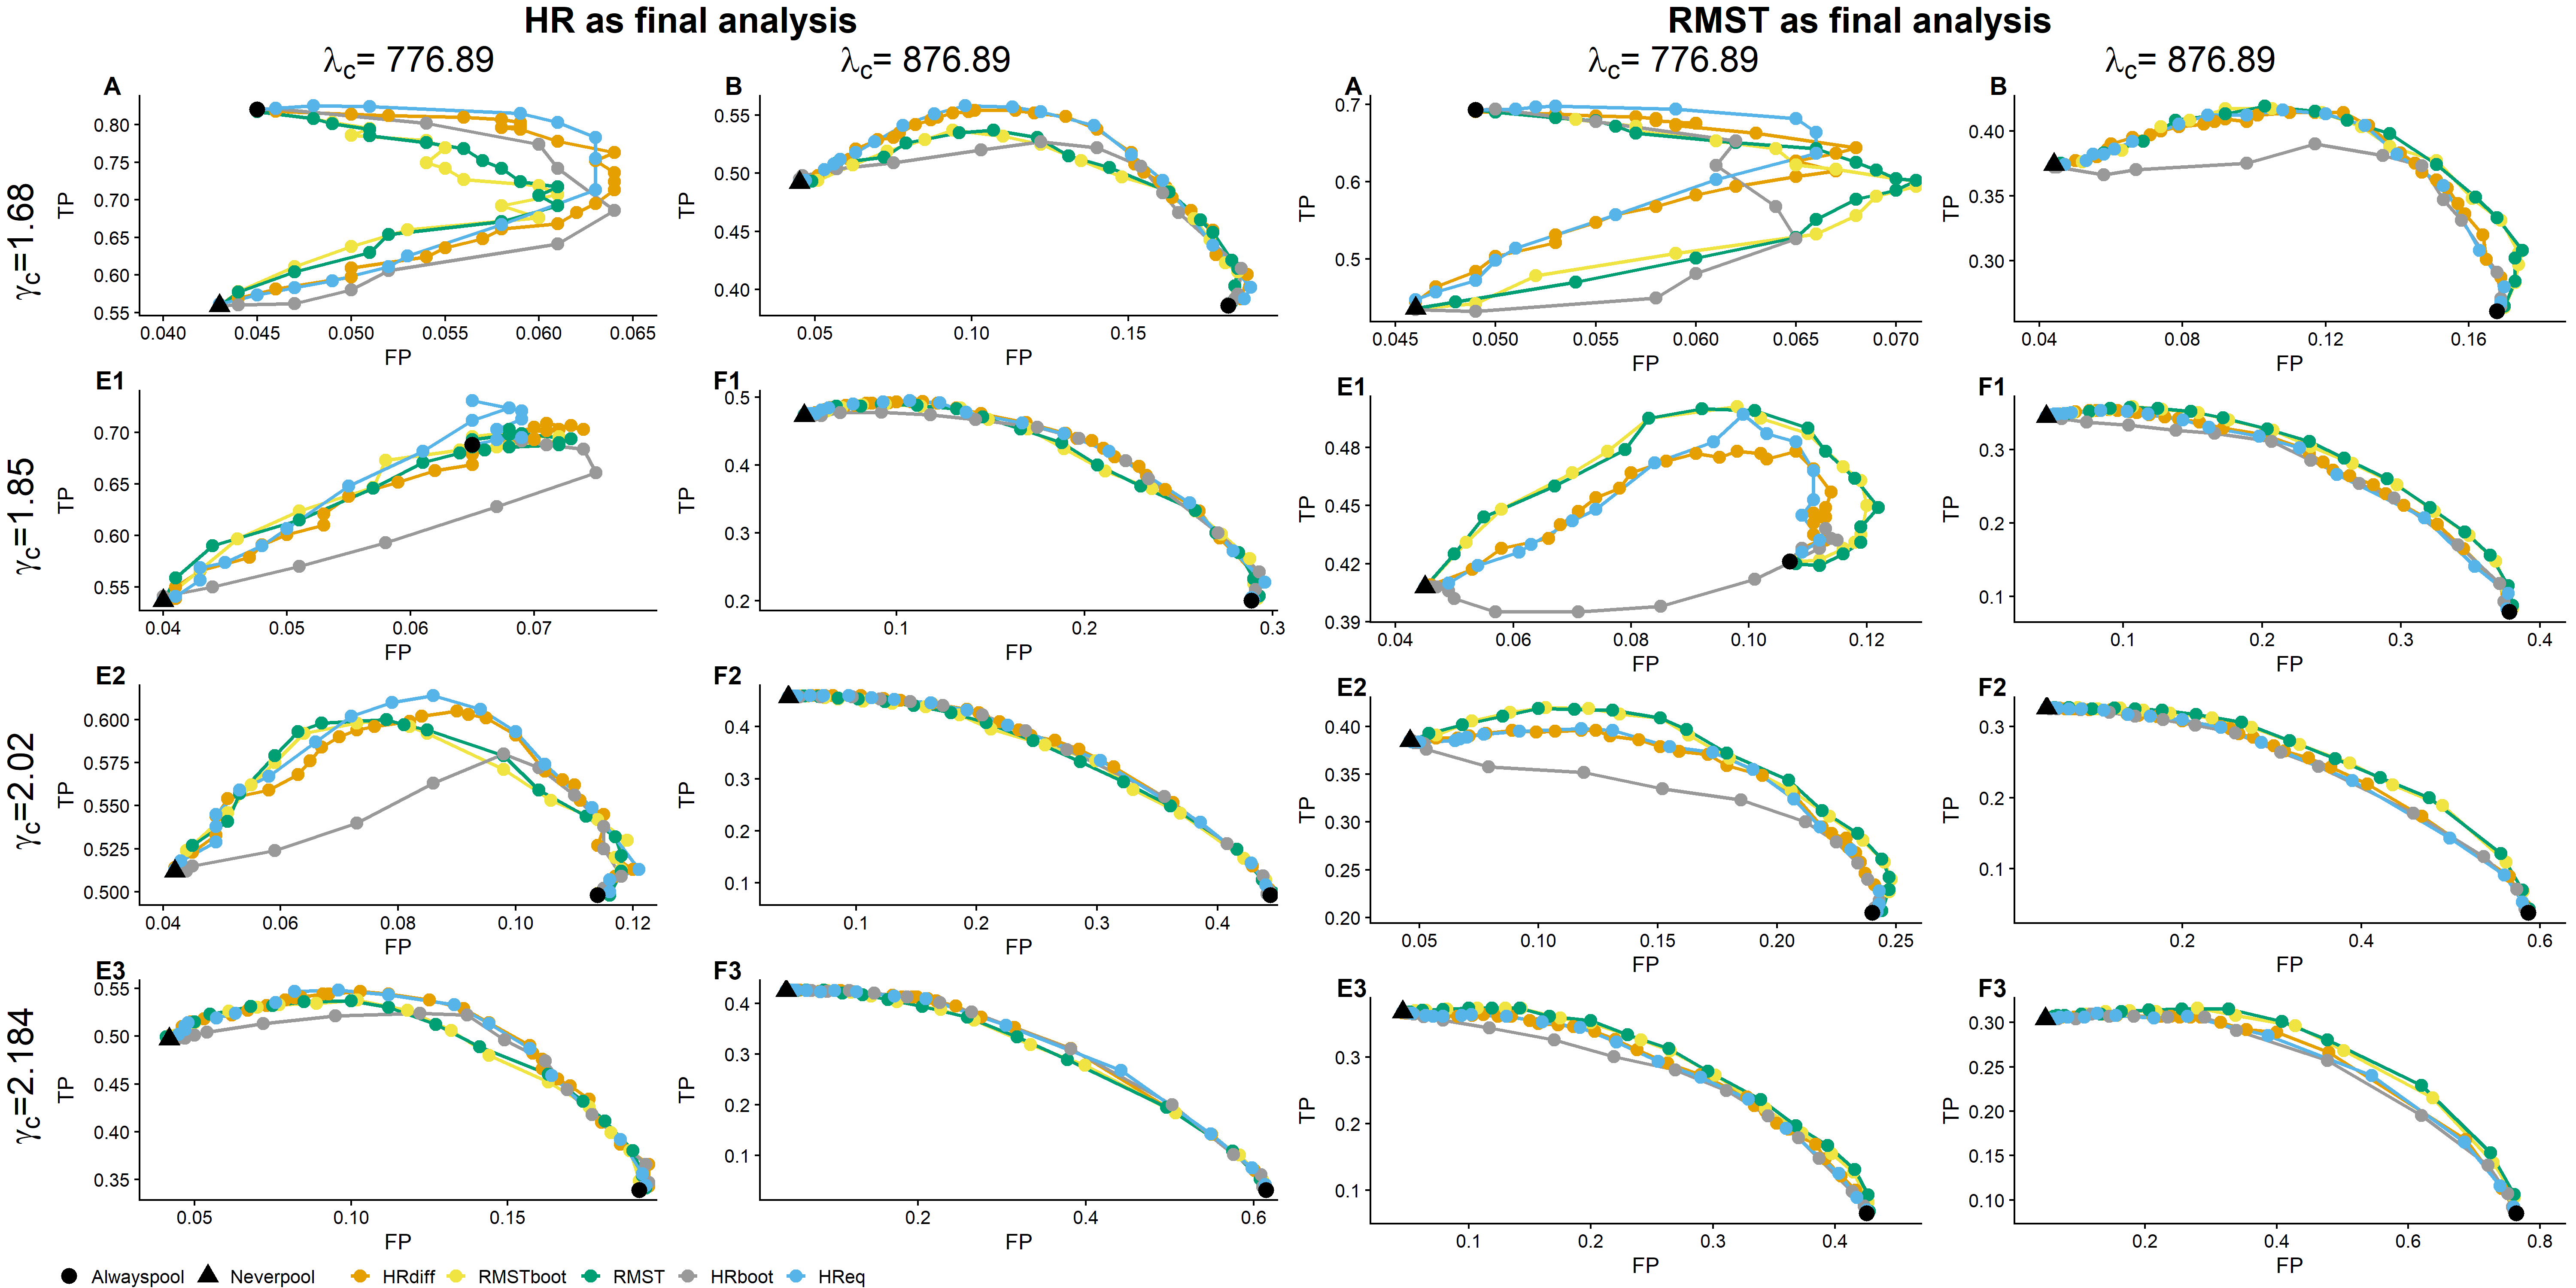
\includegraphics[width=13cm]{1.Sim2.png}
  \caption{For the simulated scenarios A, B, E1-3 and F1-3, the TPR is plotted on the y-axis, the FPR is plotted on the x-axis for the six different pooling methods. It should be noted that the scale of the x-axis and y-axis differ between the plots. The left two columns plot the operating characteristics when a HR is performed as final analysis, the right two columns plot the operating characteristics when a RMST is performed as final analysis. The input parameters for the different scenarios are indicated on the left and top of the figure. The graphs correspond with the scenarios described in table \ref{T1}, indicated in the left corner of every graph. The TPR/FPR trade-off in the situation "never pool" and "always pool" are indicated with $\triangle$ and $\bullet$ respectively.}
  \label{fig:Sim2}
\end{figure}


\subsection{Always pool vs. never pool}
\paragraph{Scenario A}
As expected, compared to "never pool" (indicated with $\triangle$ in graph \ref{fig:A-D} and \ref{fig:ScenarioA-F}), when the control groups are always pooled (indicated with $\bullet$ in the graph), the TPR greatly increases while the change in FPR is negligible. When the historical controls are always pooled, the study now reaches a power of 0.8 when a HR is performed as final analysis, and a power of 0.7 when a RMST is performed as final analysis. The FPR resembles a concave function; starting from "never pool", the TPR first increases as the FPR increases. However halfway there is a tippingpoint where the TPR starts to decrease and returns to the TPR measured at "never pool".
%However, the improvement from "never pool" to "always pool" in TPR/FPR is not linearly related to how much of the datasets are pooled. At first the FPR increases for every pooling method. Each method shows a tippingpoint where the FPR starts to decrease back to the startingpoint. It should be noted however the the scale of the y-axis is different from the scale on the x-axis. The largest FPR measured is around 0.065 for HR as final analysis, and around 0.071 for RMST as final analysis, while the gain in power is substantially more. 

\paragraph{Scenario B}
In scenario B, $\lambda_{c} > \lambda_{h}$. As expected, when the control groups are always pooled the TPR decreases and the FPR increases compared to "never pool". The loss of power is again not linearly related to the amount of control groups pooled; the TPR increases slightly before decreasing. 

\paragraph{Scenario C1-3}
Scenario C1, C2 and C3 range from smaller to larger between study variance of $\lambda_{c}$. As predicted, both the TPR and FPR increase when the control groups are always pooled compared to "never pool". While the increase in FPR is positively related to the size of the between study variance, the increase in TPR is negatively related to the size of the between study variance. In the always pool case the FPR in C3 is more than three times as large compared to the FPR in C1.

\paragraph{Scenario D1-3}
In scenario D $\lambda_{c} > \lambda_{h}$ and D1, D2 and D3 range from smaller to larger between study variance of $\lambda_{c}$.  When the control groups are always pooled the TPR decreases and the FPR increases for scenario D1 and D2. Scenario D3 shows a very small increase in TPR. The loss of power is again not linearly related to the amount of control groups pooled; the TPR increases slightly before decreasing. 

\paragraph{Scenario E1-3}
In scenario E $\gamma_{c} > \gamma_{h}$ and E1, E2 and E3 range from a smaller difference to a larger difference. When $\gamma_{c}$ increases compared to $\gamma_{h}$, the FPR increases and the TPR decreases if the control groups are always pooled compared to never pooled. Again, the decrease in TPR is not linear; it goes up before it eventually decreases. 

\paragraph{Scenario F1-3}
In scenario F $\lambda_{c} > \lambda_{h}$ and $\gamma_{c} > \gamma_{h}$. F1, F2 and F3 range from a smaller difference to a larger difference in $\gamma$. As predicted, always pooling leads to an even bigger decrease in TPR and increase in FPR compared to the scenarios C1, C2 and C3. The decrease in TPR is more linear compared to the other scenarios.

\subsection{The effect of the different pooling methods on the TPR/FPR trade-off}
To obtain further insight in what happens between "never pool" and "always pool", the TPR/FPR rate is plotted for the different pooling methods with on the x-axis the proportion of the simulated control groups pooled. Those graphs are presented in Appendix \ref{A:additionalgraphs}. In the graphs the TPR/FPR of "never pooled" is indicated by a dashed line in the plot, while the TPR/FPR of "always pooled" is indicated by a solid line in the plot. Not surprisingly, the TPR/FPR decreases with pooling when the historical controls are not commensurate (which is the case for the scenario B-F). However, what happens in the perfect world scenario (scenario A) is more interesting, hence the plots of scenario A are presented in figure \ref{fig:Aprop}. 
\begin{figure}[h!]
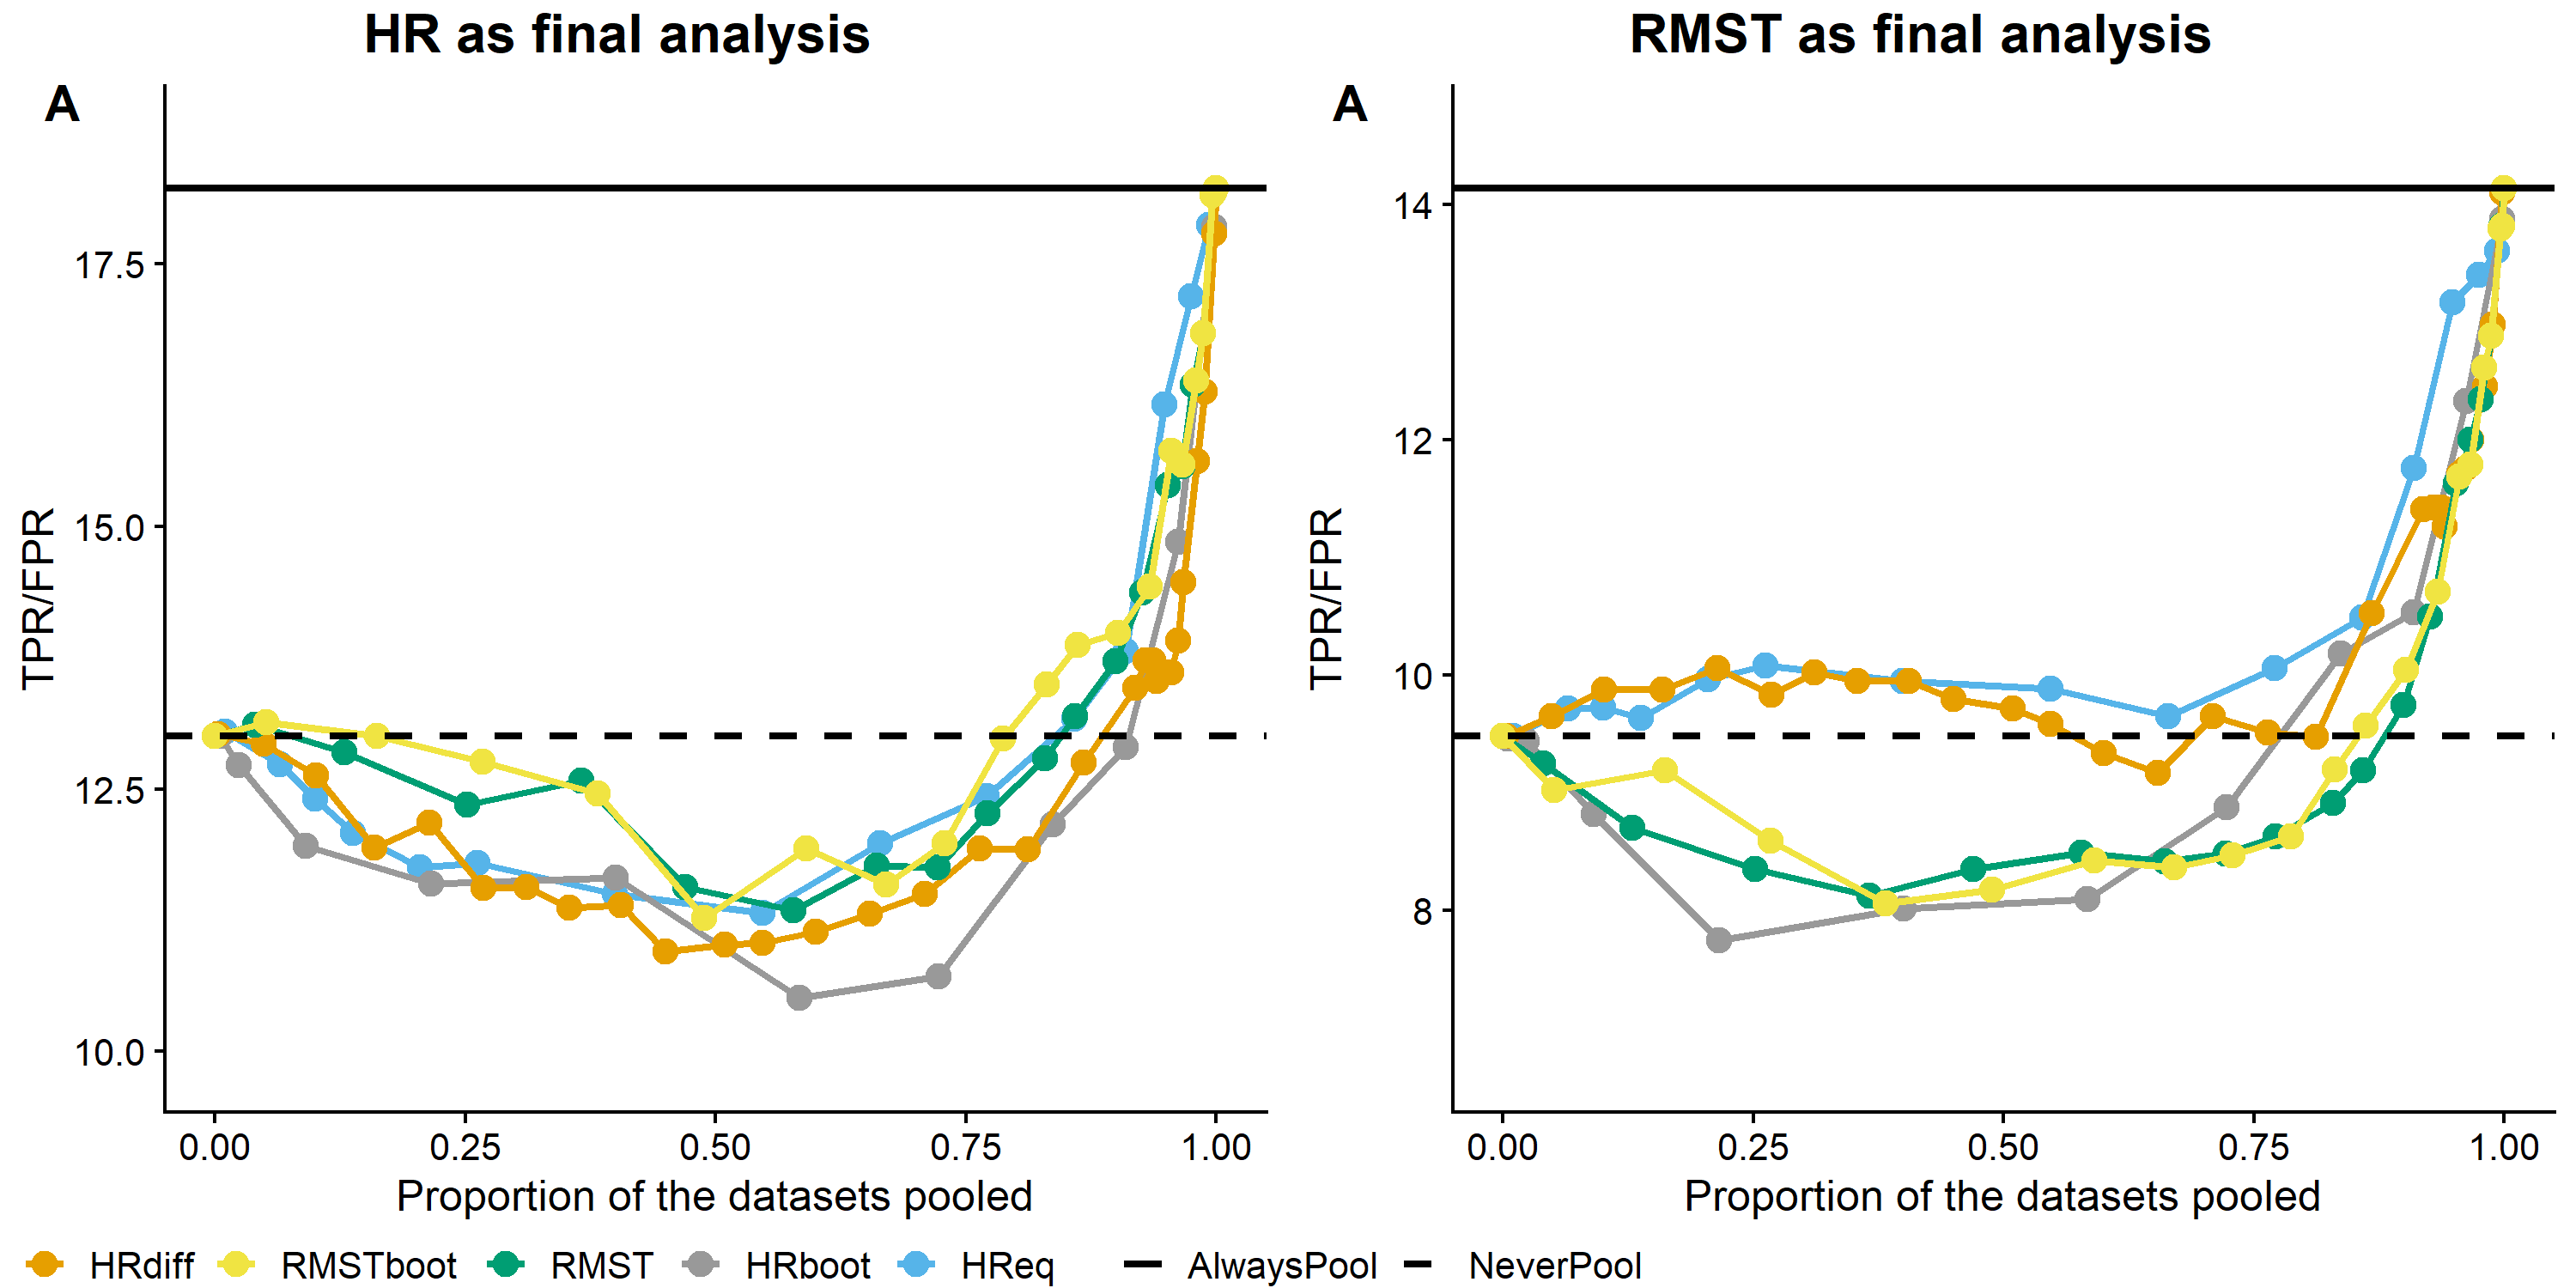
\includegraphics[width=12cm]{A.png}
  \caption{The TPR/FPR for the different pooling methods in a perfect world scenario. The TPR/FPR rate is plotted for the different pooling methods with on the x-axis the proportion of the simulated control groups pooled The TPR/FPR of "never pooled" is indicated by a dashed line in the plot, while the TPR/FPR of "always pooled" is indicated by a solid line in the plot.}
  \label{fig:Aprop}
\end{figure}
\\
When a hazard ratio test is applied as final analysis, the TPR/FPR trade-off becomes worse when a pooling method is applied compared to ignoring the historical controls completely. Only when the decision threshold implies that almost all the simulated scenarios are pooled, the TPR/FPR increases compared to "never pool". When an RMST test is applied as final analysis, the TPR/FPR of the HR difference test and HR equivalence test show a small improvement compared to "never pool". However, the TPR/FPR of the RMST methods in the right graph are still lower compared to the TPR/FPR of "never pool" in the left graph. 

\subsection{HR equivalence vs. HR difference}
In scenario A and B, the HR equivalence test has a slightly better TPR/FPR trade-off and type I error control than the HR difference method. When the between-study variance increases (scenario C1-C3 and D1-D3), the curve of HR equivalence is clearly closer to the top left corner, indicating a better TPR/FPR trade-off. However, taking into account the scale of the y-axis, the difference in TPR given a fixed FPR is still small. When the difference in shape parameter increases (scenario E1-E3 and F1-F3), the difference in TPR/FPR is less evident. 

\subsection{Bootstrapping}
In every simulated scenario, the HR equivalence test with bootstrapped CIs under performs the regular HR equivalence test. In some scenarios, the TPR/FPR trade-off of the HR equivalence test with bootstrapped CIs starts lower than that of the HR difference test near "never pool", but has a better TPR/FPR trade-off compared to the HR difference test near "always pool".     

Whereas there the bootstrapped HR equivalence test clearly under performs the regular HR equivalence test, there is no clear difference in the TPR/FPR trade-off regarding the RMST equivalence test and RMST equivalence test with bootstrapped CIs.

\subsection{RMST or HR based pooling methods}
When a HR test is performed as final analysis, the RMST based methods in scenario A, C1-3 and E1-E2 are slightly closer towards the top left corner near "never pool", indicating a better TPR/FPR trade-off for the stricter decision thresholds. However, when the decision thresholds become less strict and start approaching "always pool", the HR based methods have a better TPR/FPR trade-off. 

When a RMST test is performed as final analysis, the HR equivalence test and HR difference test clearly outperform the RMST based methods and HR equivalence boot in scenario A, C1-3 and D1-3; they show a better TPR/FPR trade-off and type I error control. HR equivalence boot starts with the lowest TPR/FPR trade-off near never pool, but performs better than the RMST based methods when approaching "always pool". In scenario B, E1-3 and F1-3 the curves of the RMST based methods are on top, but also curved towards the top right corner. The RMST based methods have a higher TPR rate and a better TPR/FPR trade-off except near "always pool", where the FPR is better controlled by the HR based methods.

\subsection{HR or RMST as Final analysis}
Compared to the HR as final analysis, the power of the RMST test as final analysis is lower. The maximum power when you would always pool in situation A is under $65\%$, compared to $80\%$ for the HR difference test. The maximum observed FPR is higher when the RMST is performed as final analysis. Surprisingly, when the assumption of proportional hazard doesn't hold, the HR difference test as final analysis clearly outperforms the RMST test as final analysis. The TPR is generally higher and the FPR is generally lower when a HR test is performed as final analysis. 

\section{Discussion}
In this study the operating characteristics of equivalence testing and bootstrapping methods for assessing the pool-ability as opposed to the more traditional test-than-pool (difference test) have been evaluated in the context of a working example. 

As predicted, the equivalence test outperforms the difference test regarding the TPR/FPR trade-off when the heterogeneity of the current controls and historical controls increases. However, the observed discrepancy between the operating characteristics of the equivalence and difference test is small. This is understandable because the decision qualities of these tests will only differ in one specific situation, namely when there is not enough power to detect a difference while there is actually a difference present. As opposed to a TTP test, an equivalence test will make the decision not to pool, because there is probably not enough power to indicate practical equivalence (depending on the range of equivalence). In other situations the decision qualities will be equally good. Along with the arguments "statistical difference does not indicate clinical relevance" and the problem of reproducibility and transparency of $p$-values as discussed in the introduction, we conclude that equivalence testing is a better fit for evaluating the pool-ability then a difference test. We acknowledge that specifying a region of practical equivalence is not always straightforward. How to specify a range of practical equivalence is outside the scope of this paper, however we do want to emphasize that when applying difference testing a "difference-threshold" is specified as well, although implicitly. \\

Furthermore, our results confirm the expected confirmation bias as a result of cherry-picking. Even in a "perfect world scenario" where the current and historical controls come from the same sampling distribution, the type I error inflates and the TPR/FPR trade-off deteriorates when the pooling methods are applied. As discussed in the introduction, by only pooling data sets that are very similar, the variation in the sampling distribution is underestimated which leads to an increase in both power and type I errors. Current controls whose estimates are by chance far away from the true population parameters, that would likely result in false positives or false negatives, are the last ones to get corrected by pooling. When the decision thresholds become less strict, the negative effect of cherry-picking fades away and the TPR/FPR trade-off starts to improve. This happens when more and more unlucky samples get a chance to get corrected by pooling, and when the estimated standard errors of the pooled datasets become more representative of the true sampling distributions. 
Hence these pooling methods do not result in relatively better decision qualities compared to ignoring historical controls completely. This is not to say that these pooling methods are always useless in practice. In some cases, when there are no alternatives, an increased type I error could be tolerated in exchange for sufficient power. But they should be used with caution and avoided when possible.
\\

Unfortunately, based on these results bootstrapping does not seem to prevent cherry-picking. The HR equivalence test with bootstrapped CIs under-performed the regular HR equivalence test. A possible explanation is that the assumptions of proportional hazards is not met for many bootstrapped samples, even in a perfect world scenario where the shape parameters of the populations are simulated to be equal. If we would estimate the shape and scale parameters for the bootstrapped samples, both parameters will vary across samples. As discussed before, if the shape parameter differs between the current and historical control group, the hazard ratio and its confident interval are difficult to interpret because they do not fully capture the difference in survival time. 
This is not the case for the RMST tests, as the RMST does not rely on the assumption of proportional hazards. The FPR/TPR trade-off seems to be almost equal for RMST and RMST boot in all simulated scenarios. This might be the result of the following; samples that are not very representative of their population can be divided into two groups; they either lead to a higher probability of finding a true/false positive result or a lower probability of finding a true/false positive result. Because bootstrapping will correct both cases equally well, the trade-off FPR/TPR does not change.
\\

Based on these results, we cannot provide readers with a definite answer about whether a RMST or HR based pooling method is more appropriate to use. This depends on the situation and type of final analysis applied.
Although not part of our research question, it might be of interest to the reader to note that the RMST as final analysis resulted in both lower power and an increased type I error compared to the HR test in situations where the proportional hazards assumption did not hold.
\\

Furthermore, the chosen effect size in the experimental group and the sample sizes of both the current controls and historical controls influence the obtained results. Although the differences between the pooling methods would become less or more visible with different settings, we do not expect that the conclusions as described in this paper would be influenced by these alternative settings.\\

There are some important considerations we left untouched.
In this simulation study only the current control group is varied. We have treated the historical control as static and representative of the historical target population because of the enormous sample size. It is however important to realize that, especially when the sample size of the historical control group is smaller, the historical controls also come from a sampling distribution that could deviate from the target population due to sampling variance and between study variation.\\

Previous literature has also proposed "dynamic borrowing" that let the degree of borrowing depend on the compatibility of the current and historical controls to mitigate the risk of bias and inflated type I error.\cite{viele2014} We believe that a researcher should only pool when (s)he is convinced that the control groups are compatible enough to pool. Partly pooling when the researcher is unsure about the compatibility will lead to increased type I errors in the long run. In the simulation study we either pooled the control groups completely or not at all. The result is that when the decision is made to pool, the sample size of the historical control group greatly outnumbers the sample size of the current control group. This also leads to highly unbalanced sample sizes of the (pooled) control group and experimental group in the final analysis. One could also consider weighting the historical control group or randomly sampling from it to reduce the dominance of the historical control group in the final analysis.\\  

Another question that we did not address is whether the power-calculations should be performed for a test without pooling, or whether the historical controls should be concluded in the study-planning. Furthermore when a certain precision level is targeted, the design of a trial that incorporates historical controls can be made more statistically efficient by incorporating unequal randomization between control and intervention group in the planning of the trial, reducing the required sample size.\cite{dron2019} Perhaps an interim analysis is needed to make a decision about the required sample size and whether unequal randomization can be applied for the remaining participants. Although outside the scope of this article, these are practical questions that should be addressed in further research. \\

In this study the emphasis was on comparing the operating characteristics of different pooling methods. In order to make a fair comparison across the methods we did not incorporate the region of practical equivalence in the final analysis. If the region of practical equivalence is also considered in the final analysis (as it should, according to the definition of the region of practical equivalence), the difference between the pooled control group and the experimental group is only deemed significant when the region of practical equivalence is not captured within or overlaps with the CI. To control the type I error, the null-value that corresponds to the null hypothesis is simply replaced with the range of values that span the specified region of practical equivalence. This does however emphasize the importance of carefully specifying a "range of practical equivalence" and precise sample size calculations, because sufficient power is needed for the equivalence test to pool (the CI should be contained within the range of practical equivalence) and to perform the final analysis (the CI should be completely outside the range of practical equivalence). This is a fine balance, because a broader region of practical equivalence will lead to a higher probability of pooling, but a lower probability of concluding that there is an effect present in the final analysis. \\

Furthermore, an interesting topic to look into is testing the practical equivalence of prognostic factors or propensity scores as opposed to testing the equivalence of the parameter evaluated in the final analysis. This would be a form of minimization, where the balance between groups for a range of prognostic factors is ensured.\cite{chio2009} This could be an interesting alternative because the decision to pool or not is not one-to-one related to the parameter in the final analysis. Perhaps this could (partly) prevent the conformation bias that results from cherry-picking.\\

With this article we trust to have convinced researchers that equivalence testing is a more appropriate measure for testing the pool-ability of current and historical controls than difference testing. More research is needed regarding the application of the equivalence test in practice. Furthermore, we want to highlight the problem of "cherry-picking" and the resulting type I error inflation. Unfortunately, this is a problem that has not yet been solved and will remain an important issue when considering pooling historical controls in a current study.  

\begin{acks}
I would like to thank the Julius centre Utrecht for providing me with the opportunity to work on this project. Specifically, I would like to express my appreciation towards my supervisors Dr. K. Oude Rengerink and Prof. Dr. K.C.B. Roes for their guidance, feedback and support throughout my master thesis project. Additionally, I would like to thank Dr. R. van Eijk for his valuable input and expertise regarding ALS trials.
\end{acks}

\begin{dci}
The Author declares that there is no conflict of interest.
\end{dci}

%Data availability statement
\bibliographystyle{SageV} 
\bibliography{BIBTEXfile}

\appendix 
\section{Appendix} 
\subsection{Poolingcriteria \label{A:Poolingcriteria}}

\begin{table}[H]
%\small\sf\centering
\caption{Decision thresholds applied in the simulation study \label{Table:DecisionCriteria}}
\begin{tabular}{lll}
\toprule
pooling method&&Decision criteria\\
\midrule
HR diff && 0; 0.0001; 0.001; 0.01; 0.02; 0.03; 0.04; 0.05; 0.06; 0.07; 0.08; 0.09;\\
&& 0.1; 0.15; 0.2; 0.25; 0.3; 0.35; 0.4; 0.45; 0.5; 0.55; 0.6; 0.65; 0.7; 0.75; \\
&& 0.8; 0.85; 0.9; 0.95; 0.99; 0.999; 0.9999; 1\\
&&\\
HR eq && [0.00001, 1/(0.00001)];
[0.001, 1/(0.001)];
[0.01, 1/(0.01)];\\
\& HR eq boot && 
[0.1, 1/(0.1)];
[0.2, 1/(0.2)];
[0.25, 1/(0.25)];
[0.3, 1/(0.3)];\\
&& 
[0.35, 1/(0.35)];
[0.4, 1/(0.4)];
[0.45, 1/(0.45)];
[0.475, 1/(0.475)];\\
&& 
[0.5, 1/(0.5)];
[0.525, 1/(0.525)];
[0.55, 1/(0.55)];
[0.575, 1/(0.575)];\\
&&
[0.6, 1/(0.6)];
[0.625, 1/(0.625)];
[0.65, 1/(0.65)];
[0.66, 1/(0.66)];\\
&&
[0.67, 1/(0.67)];
[0.675, 1/(0.675)];
[0.68, 1/(0.68)];
[0.69, 1/(0.69)];\\
&&
[0.7, 1/(0.7)];
[0.8, 1/(0.8)];
[0.9, 1/(0.9)];
[0.999, 1/(0.999)] \\

&& \\

RMST eq && [-0; 0];
[-10; 10];
[-20; 20];
[-30; 30];
[-35; 35];
[-37.5; 37.5];
[-40; 40];\\
\& RMST eq boot && [-42.5; 42.5];
[-45; 45];
[-47.5; 47.5];
[-50; 50];
[-52.5; 52.5];
[-55; 55]; \\
&& [-57.5; 57.5];
[-60; 60];
[-62.5; 62.5];
[-65; 65];
[-67.5; 67.5];
[-70; 70]; \\
&& [-75; 75];
[-80; 80];
[-85; 85];
[-90; 90];
[-95; 95];
[-100; 100];\\
&& [-110; 110];
[-150; 150];
[-1000; 1000]

\bottomrule
\end{tabular}\\[10pt]
\end{table}

\\
\subsection{Additional graphs \label{A:additionalgraphs}} 
\begin{figure}[h!]
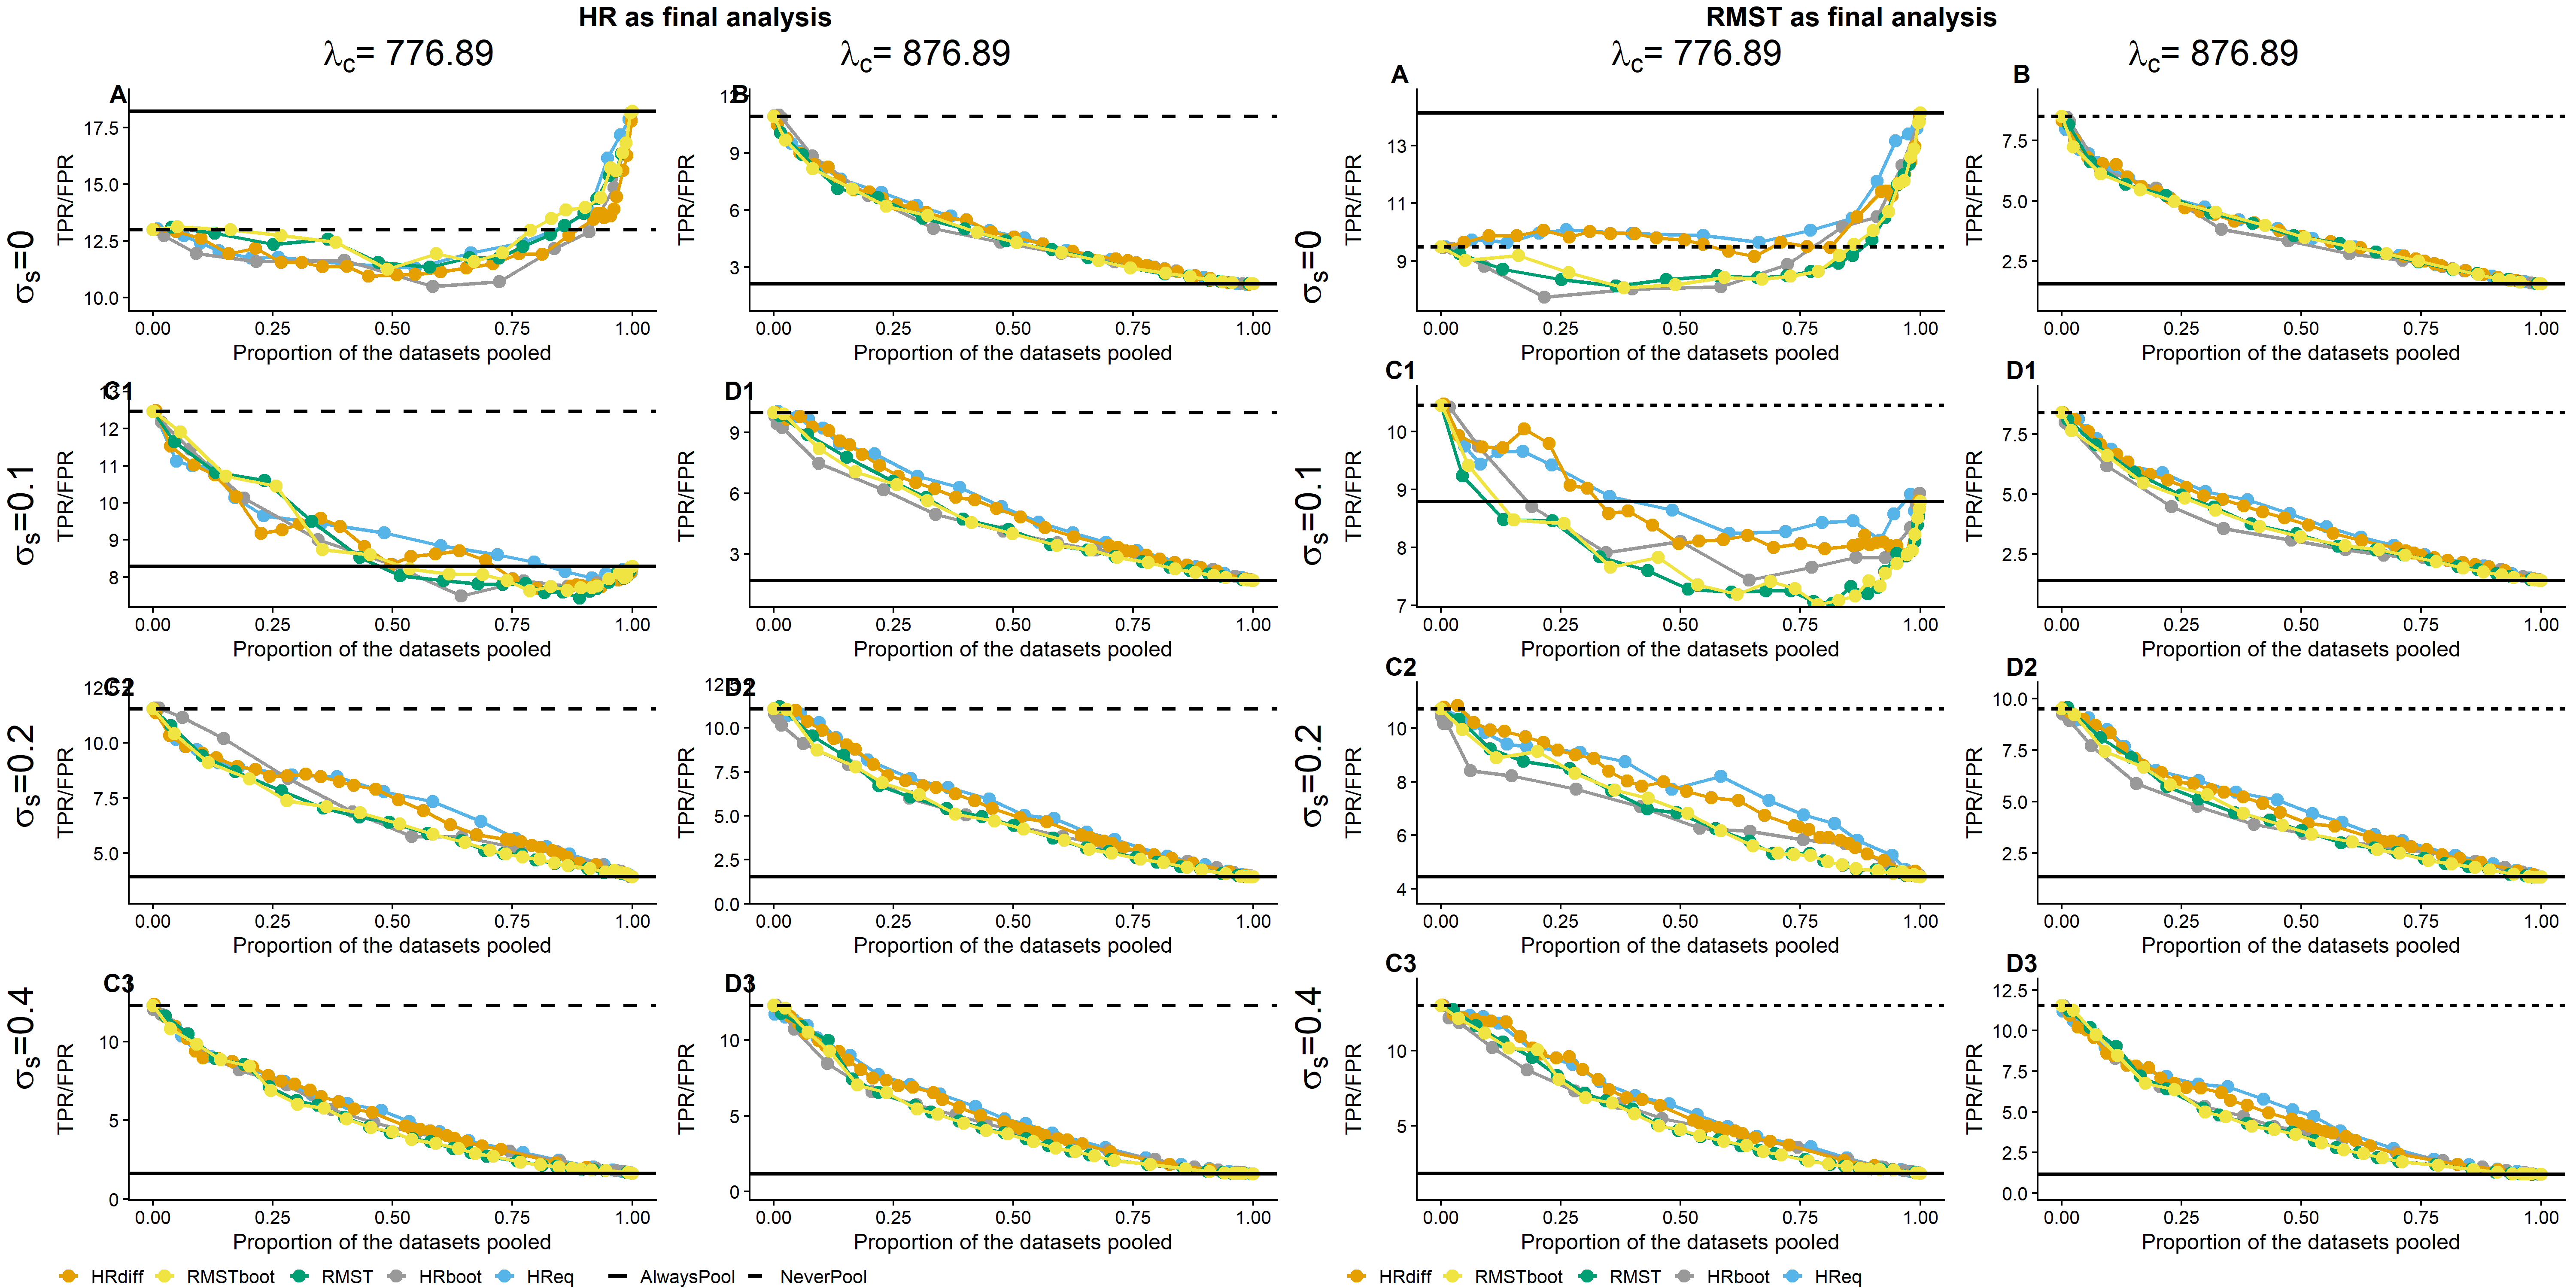
\includegraphics[width=13cm]{prop1.png}
  \caption{The TPR/FPR for the different pooling methods for scenario A - D. The TPR/FPR rate is plotted for the different pooling methods with on the x-axis the proportion of the simulated control groups pooled The TPR/FPR of "never pooled" is indicated by a dashed line in the plot, while the TPR/FPR of "always pooled" is indicated by a solid line in the plot.}
  \label{Prop1}
\end{figure}
\begin{figure}[h!]
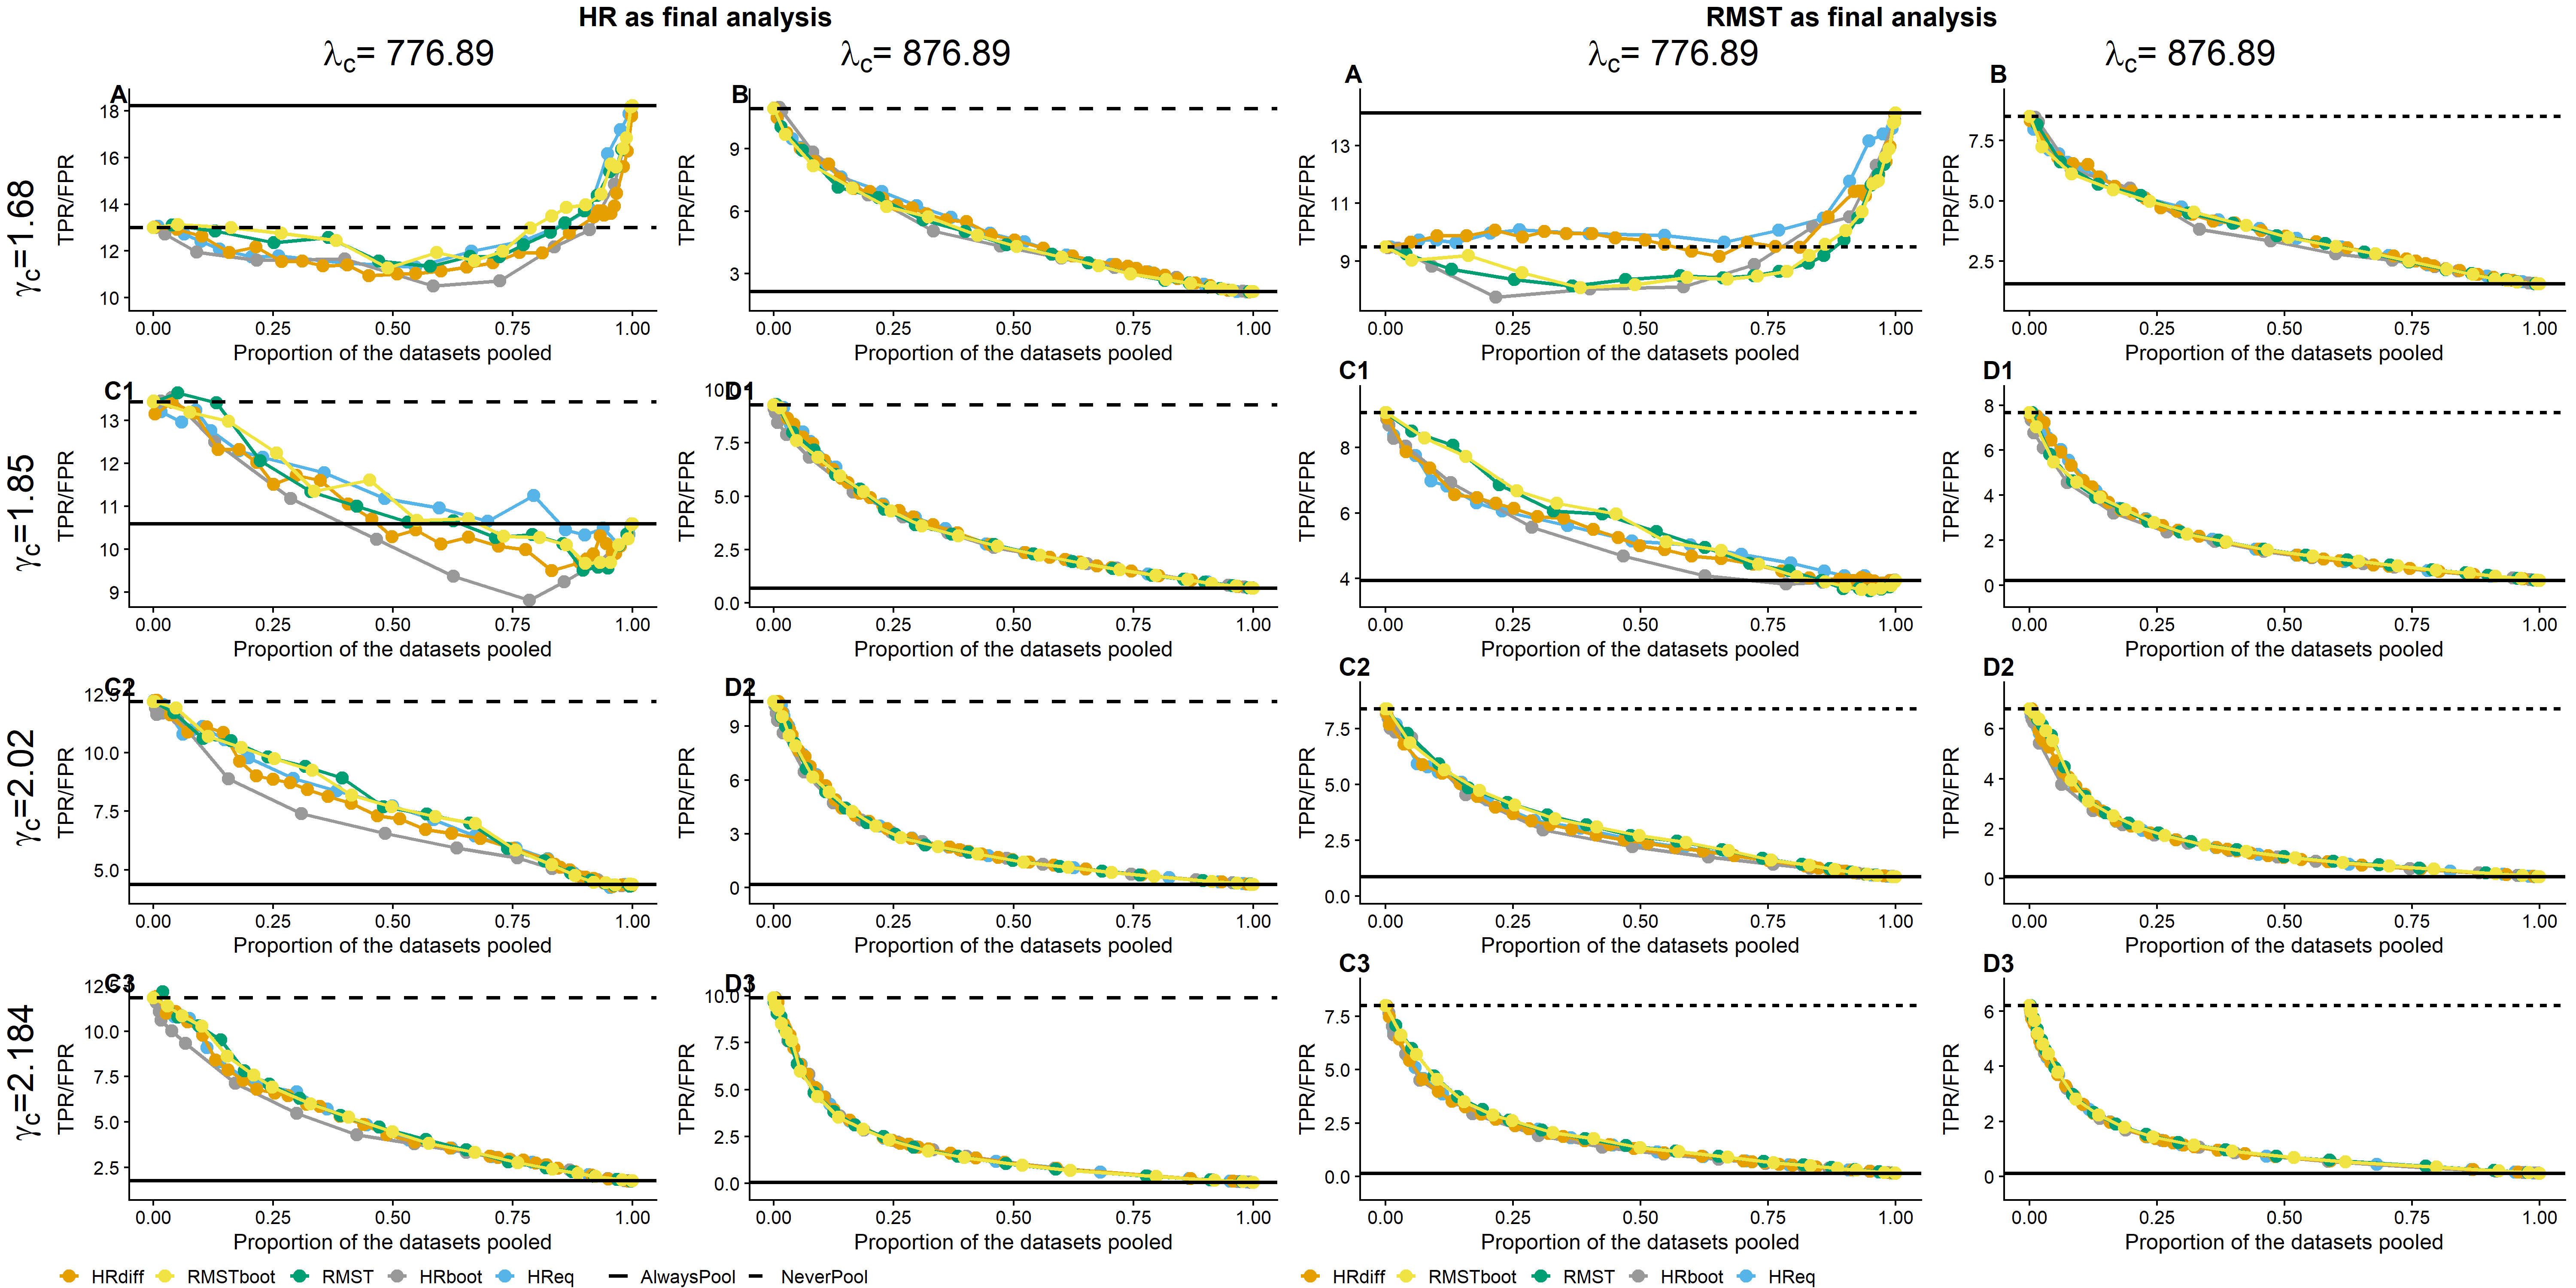
\includegraphics[width=13cm]{prop2.png}
  \caption{The TPR/FPR for the different pooling methods for scenario A, B, C1-3 and D1-3. The TPR/FPR rate is plotted for the different pooling methods with on the x-axis the proportion of the simulated control groups pooled The TPR/FPR of "never pooled" is indicated by a dashed line in the plot, while the TPR/FPR of "always pooled" is indicated by a solid line in the plot.}
  \label{Prop2}
\end{figure}



 
%To date, there are no clear guidelines how to appropriately incorporate information from the concurrent control groups in this situation (Cianci: which situation), keeping the type I error in control. This paper provides a real-life example how to incorporate information of multiple control arms when the underlying true effect parameter (explain effect parameter) can be assumed to be equal (equal to???). The gain in power and the resulting reduction is sample size is discussed. 

%Viele:
%Alternative methods such as test‐then‐pool, power priors, and hierarchical models can produce lower type I error inflation, and in fact, each of these methods has user‐settable parameters that allow the user to cap the amount of type I error inflation in a specific range of control rates.



\end{document}
